\chapter*{付録} % 章番号を出さない
\addcontentsline{toc}{chapter}{付録} % 目次に載せる

% 「付録」(appendix)は、論文の本文に載せるには情報として邪魔もしくは必須ではないものの、読者にとって有益となるような情報を載せます。付録を必要としない論文ももちろん存在しますので、そこは著者の判断です。

% 例えば、たくさんの観測データを様々なモデルでフィットした場合、フィット結果の絵がたくさん出てくるはずです。そのような図は本文中に大量に出されても大切な情報を見失ってしまいますので、大部分は付録に載せることが推奨されます。他には、何かしらの長い式変形や証明を載せる必要がある場合、付録に移動する場合があります。

% 付録は chapter の 1 つとして作りますが、章番号は表示しません。
% また付録の 1 つずつはアルファベットで番号付けをするのが一般的です。
\setcounter{section}{0} % section の番号をゼロにリセットする
\renewcommand{\thesection}{\Alph{section}} % 数字ではなくアルファベットで数える
\setcounter{equation}{0} % 式番号を A.1 のようにする
\renewcommand{\theequation}{\Alph{section}.\arabic{equation}}
\setcounter{figure}{0} % 図番号
\renewcommand{\thefigure}{\Alph{section}.\arabic{figure}}
\setcounter{table}{0} % 表番号
\renewcommand{\thetable}{\Alph{section}.\arabic{table}}

% \section{すごい長い証明}
% 式~(\ref{eq})のように、式番号がアルファベットとアラビア数字の組み合わせになるように、\LaTeX{}ソース中で設定してありますので、中身を眺めてみてください。

% \begin{equation}
%   \label{eq}
%   1 + 1 = 2
% \end{equation}


% \section{修士論文添削前に自己点検する項目}

% \begin{itemize}
% \item[\CID{00728}] 第\ref{chap:plagiarism}章を読み、剽窃について十分に理解したか。
% \item[\CID{00728}] 修士論文に剽窃箇所もしくは剽窃と見なされうる箇所は存在しないか。
% \item[\CID{00728}] \LaTeX\ で図番号などの参照先がないせいで「図??」「表??」「??節」のようになっている箇所はないか。
% \item[\CID{00728}] 日本語読点「、」と欧文カンマ「,」が混在していないか。例えば「ガンマ線望遠鏡は、HESS, MAGIC, VERITASなどがある」。
% \item[\CID{00728}] 日本語丸括弧「()」と欧文丸括弧「()」が混在していないか。
% \item[\CID{00728}] 単位と数値の間にスペースは入っているか。「100MeV」など。
% \item[\CID{00728}] 単位が斜体になっていないか。「$100~MeV$」など。
% \item[\CID{00728}] 変数でない添字などが斜体になっていないか。$N_{trigger}$など。
% \item[\CID{00728}] 自分で作成したものではない図や写真は、全て出典が明記され、転載であることを書いてあるか。
% \end{itemize}

\section{無限運動量飛跡試験に際して行われた修正}
\label{sec:appendix:infinite-momentum-tracks}
無限運動量飛跡の試験で明らかになったトリガー回路の修正点とそのデバッグの過程について述べる。図\ref{}に修正を行う前の結果を示す。トリガー回路のデバッグ前の段階では多くのInefficiencyが見られた。\ref{}章で述べたようにトリガー回路はこれまでにソフトウェアシミュレーターとVivado シミュレーターで動作検証は行われてきたが、これらのInefficiencyは大統計量を用いた網羅的な試験によって初めて発見されたものである。以下にそれぞれのモジュールにおけるInefficiencyとその解決について述べる。

\begin{figure}
  \begin{minipage}[b]{.5\linewidth}
      \centering
      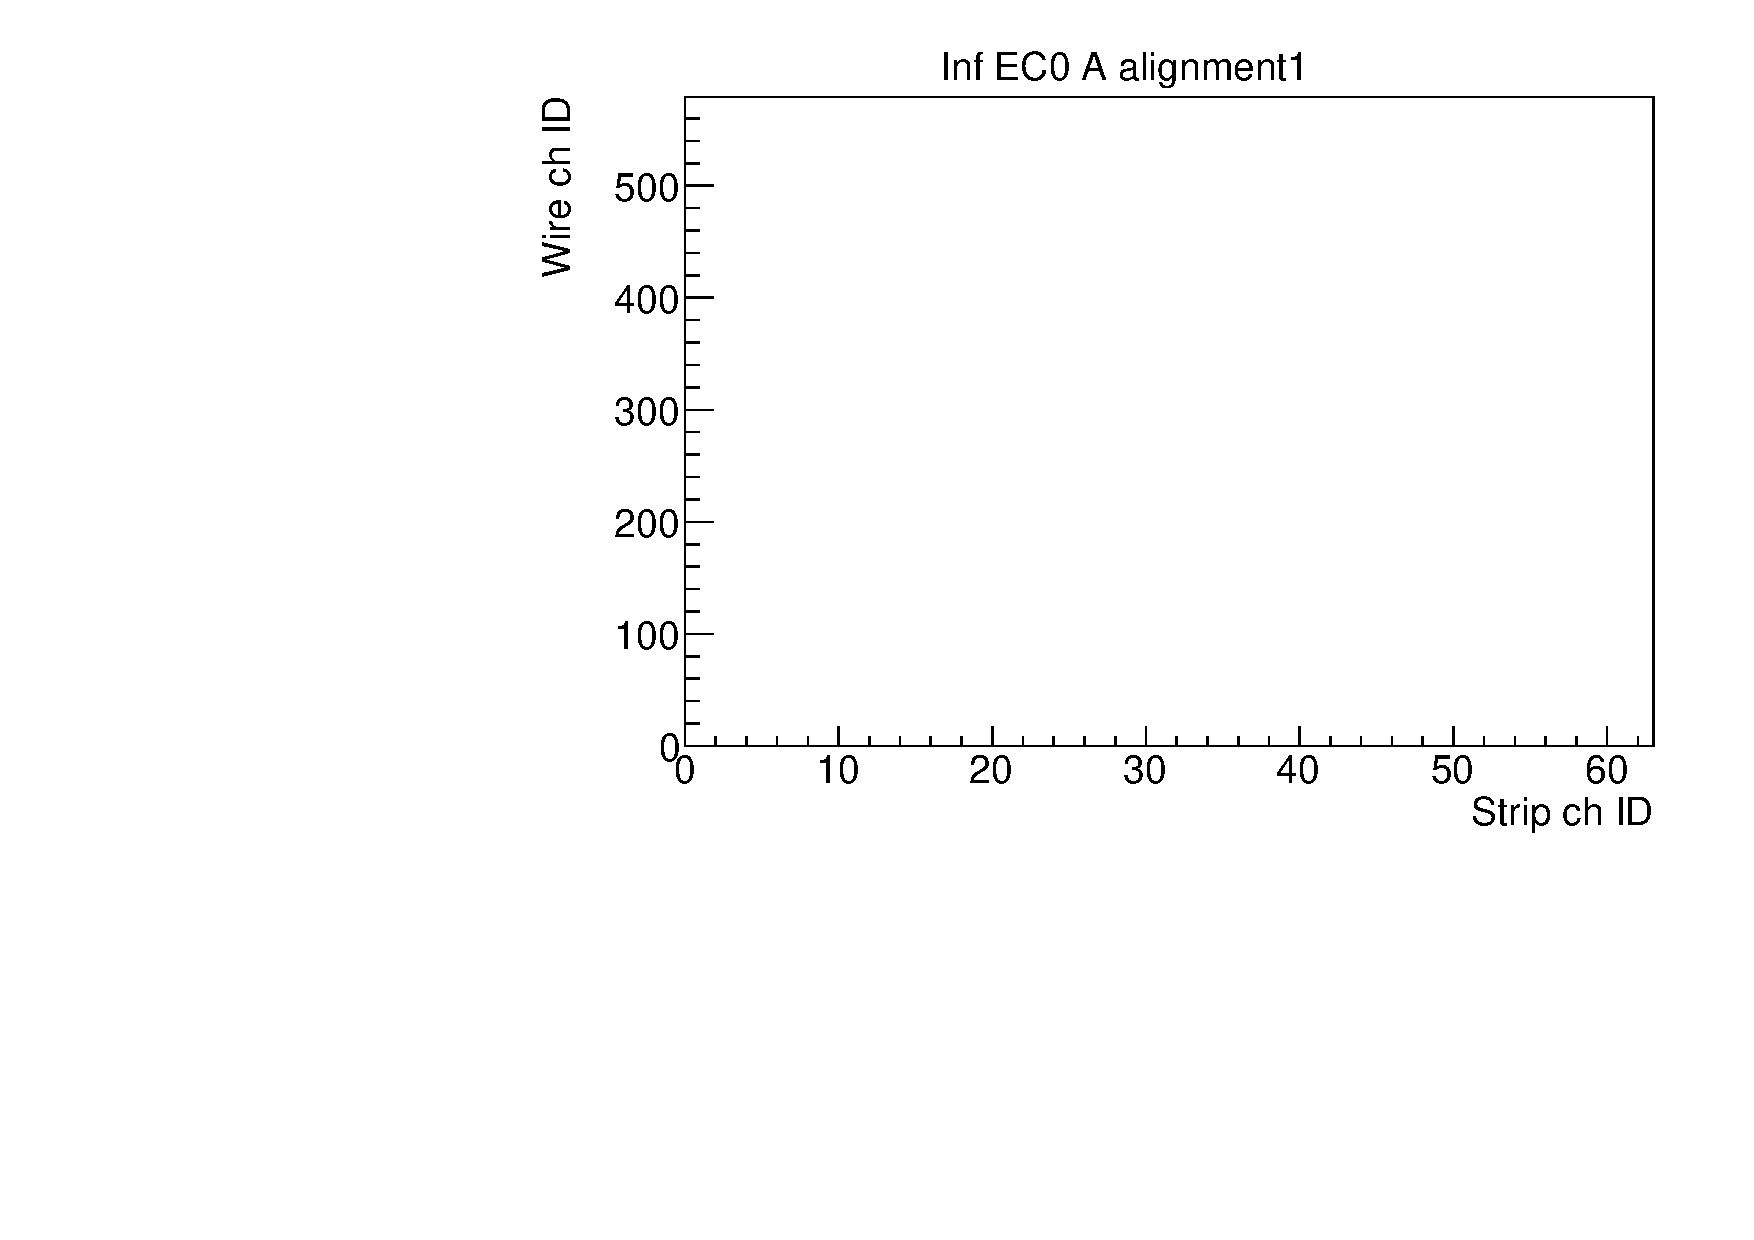
\includegraphics[height=6cm]{fig/Test/B_InfEC0_strip.pdf}
      \subcaption{エンドキャップ$\phi\,$0領域の結果}
  \end{minipage}
  \begin{minipage}[b]{.5\linewidth}
      \centering
      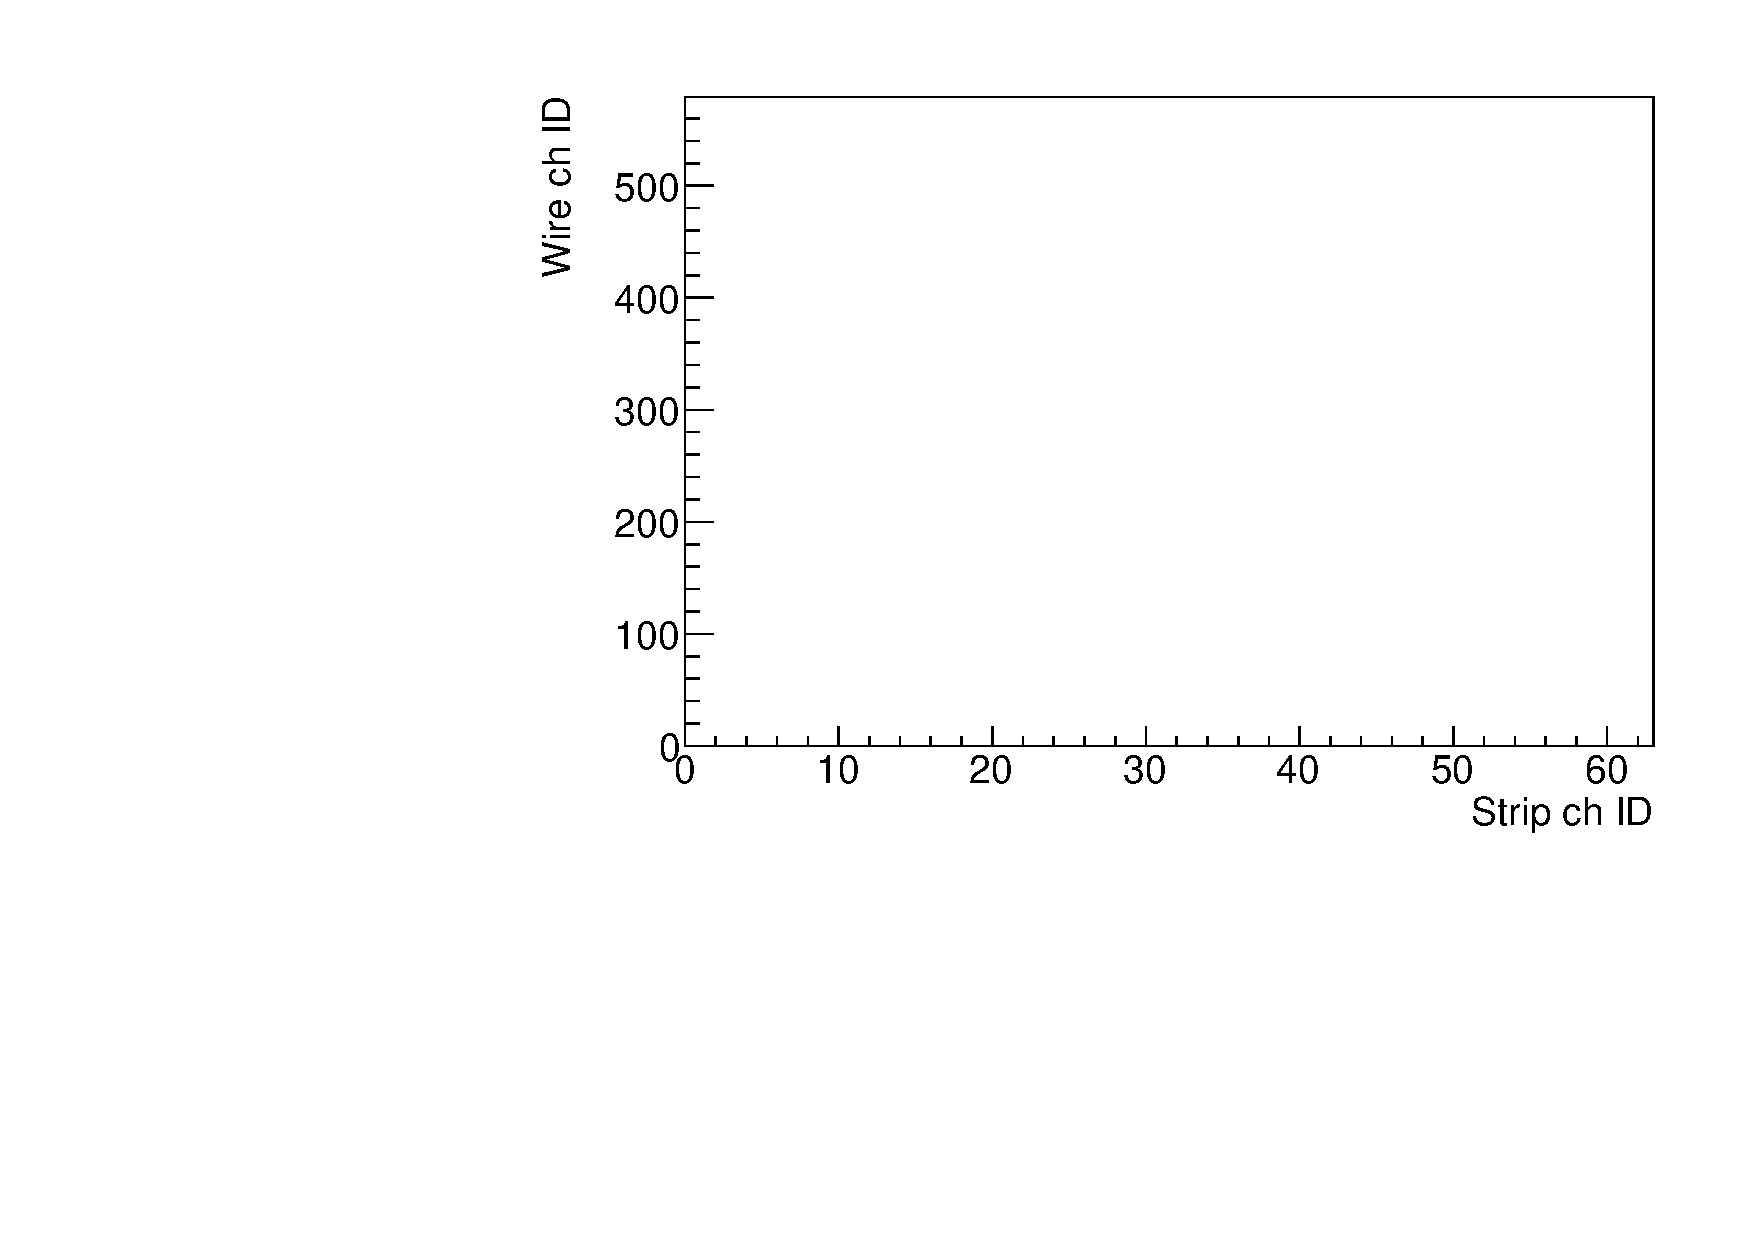
\includegraphics[height=6cm]{fig/Test/B_InfEC1_strip.pdf}
      \subcaption{エンドキャップ$\phi\,$1領域の結果}
  \end{minipage}\\
  \begin{minipage}[b]{\linewidth}
      \centering
      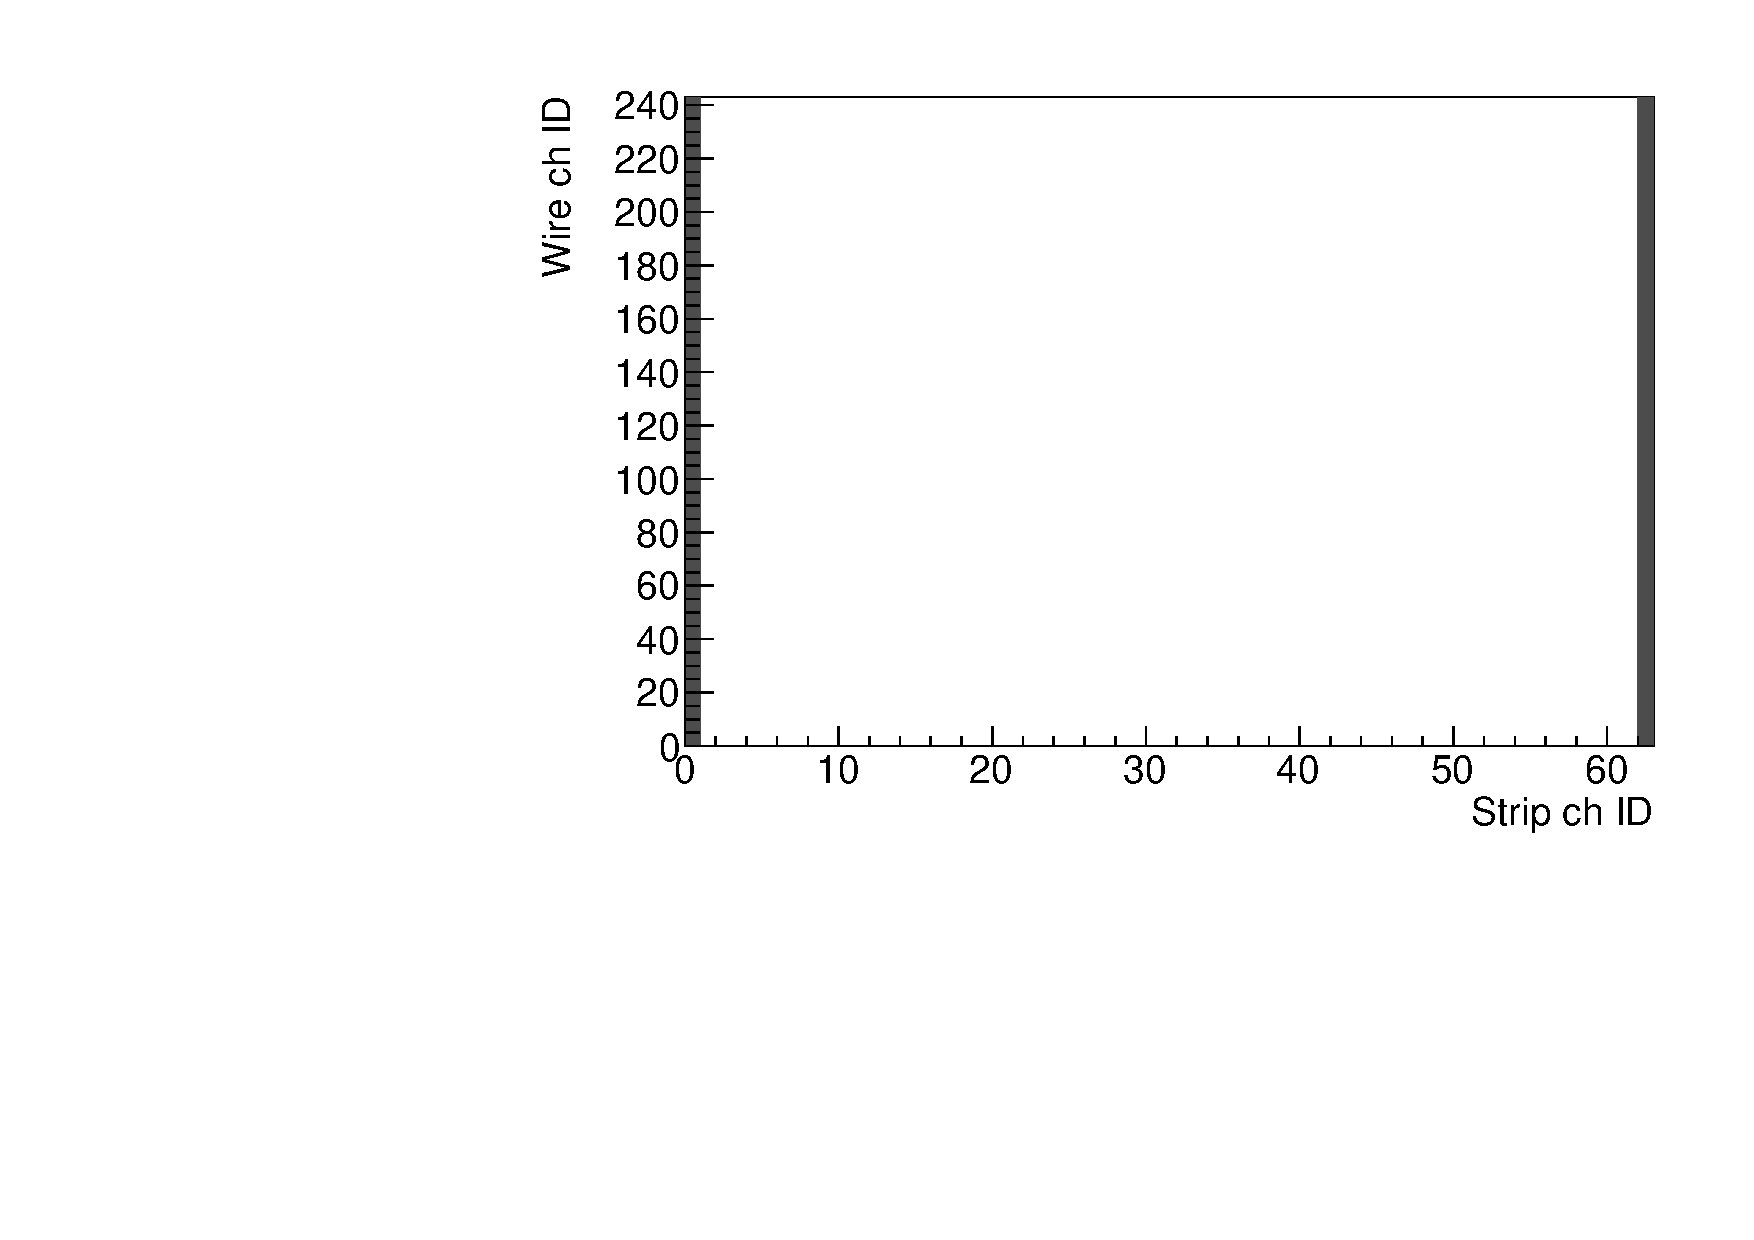
\includegraphics[height=6cm]{fig/Test/B_InfFW_strip.pdf}
      \subcaption{フォワード領域の結果}
  \end{minipage}
  \caption[異なる画像形式の比較]{無限運動量飛跡に対する、Strip Segment Reconstructionの応答。}
  \label{Inf_B_Strip}
  \end{figure}
  
  \begin{figure}
      \begin{minipage}[b]{.5\linewidth}
          \centering
          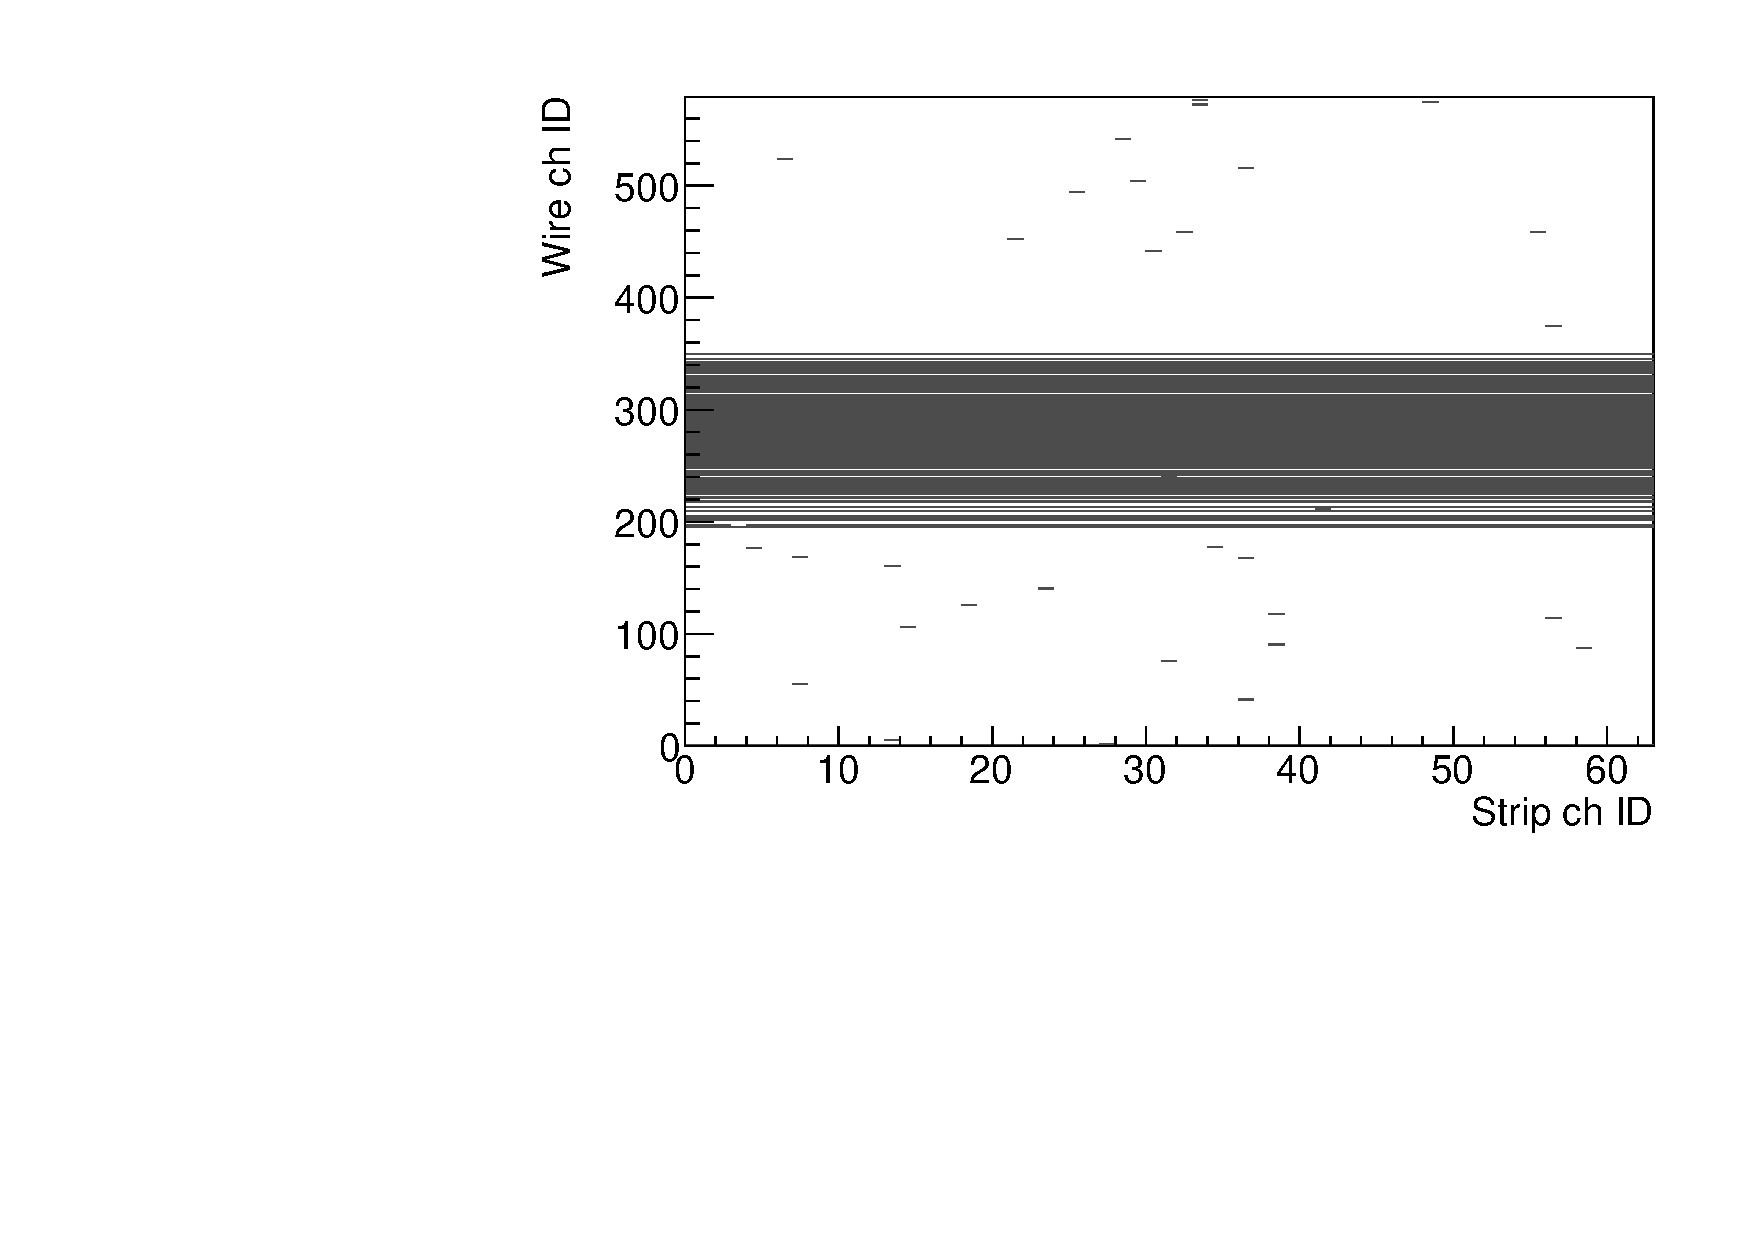
\includegraphics[height=6cm]{fig/Test/B_InfEC0_wire.pdf}
          \subcaption{エンドキャップ$\phi\,$0領域の結果}
      \end{minipage}
      \begin{minipage}[b]{.5\linewidth}
          \centering
          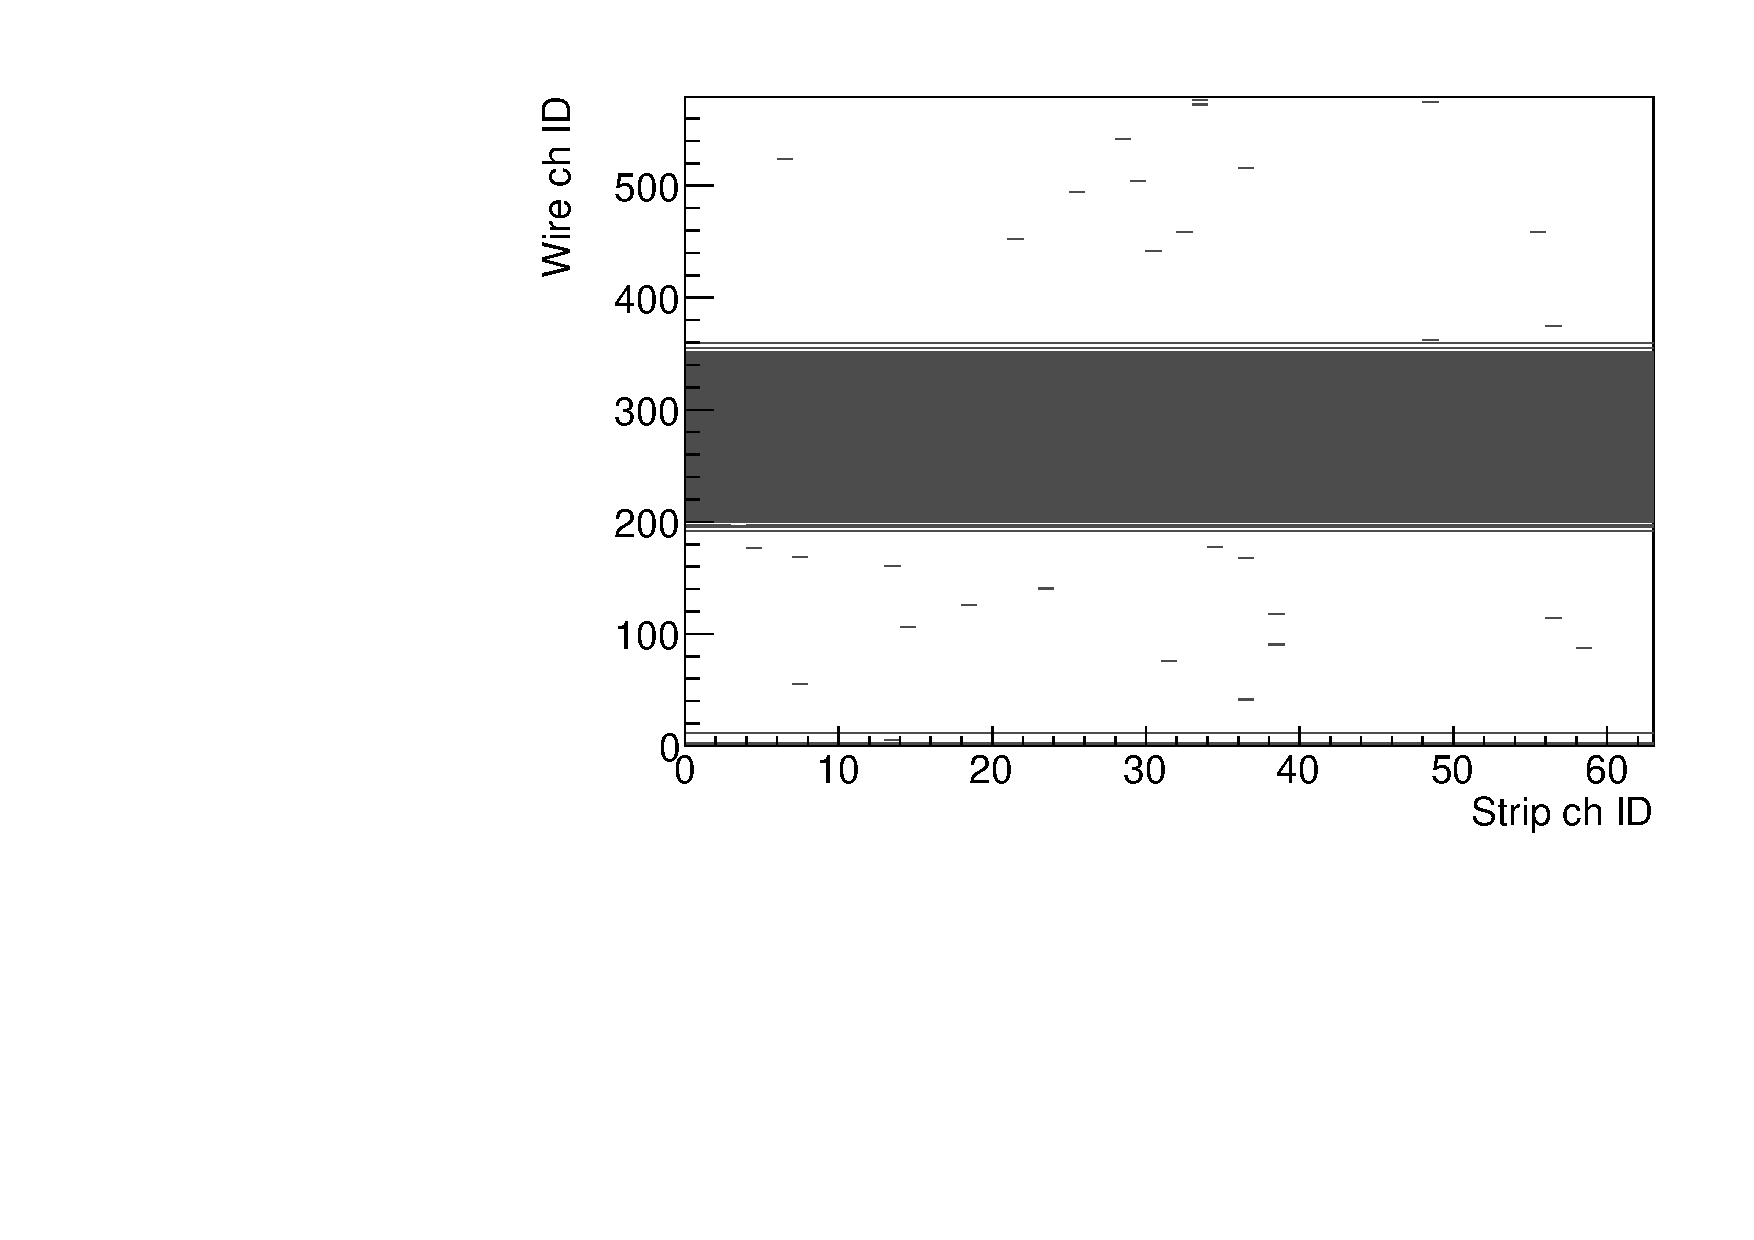
\includegraphics[height=6cm]{fig/Test/B_InfEC1_wire.pdf}
          \subcaption{エンドキャップ$\phi\,$1領域の結果}
      \end{minipage}\\
      \begin{minipage}[b]{\linewidth}
          \centering
          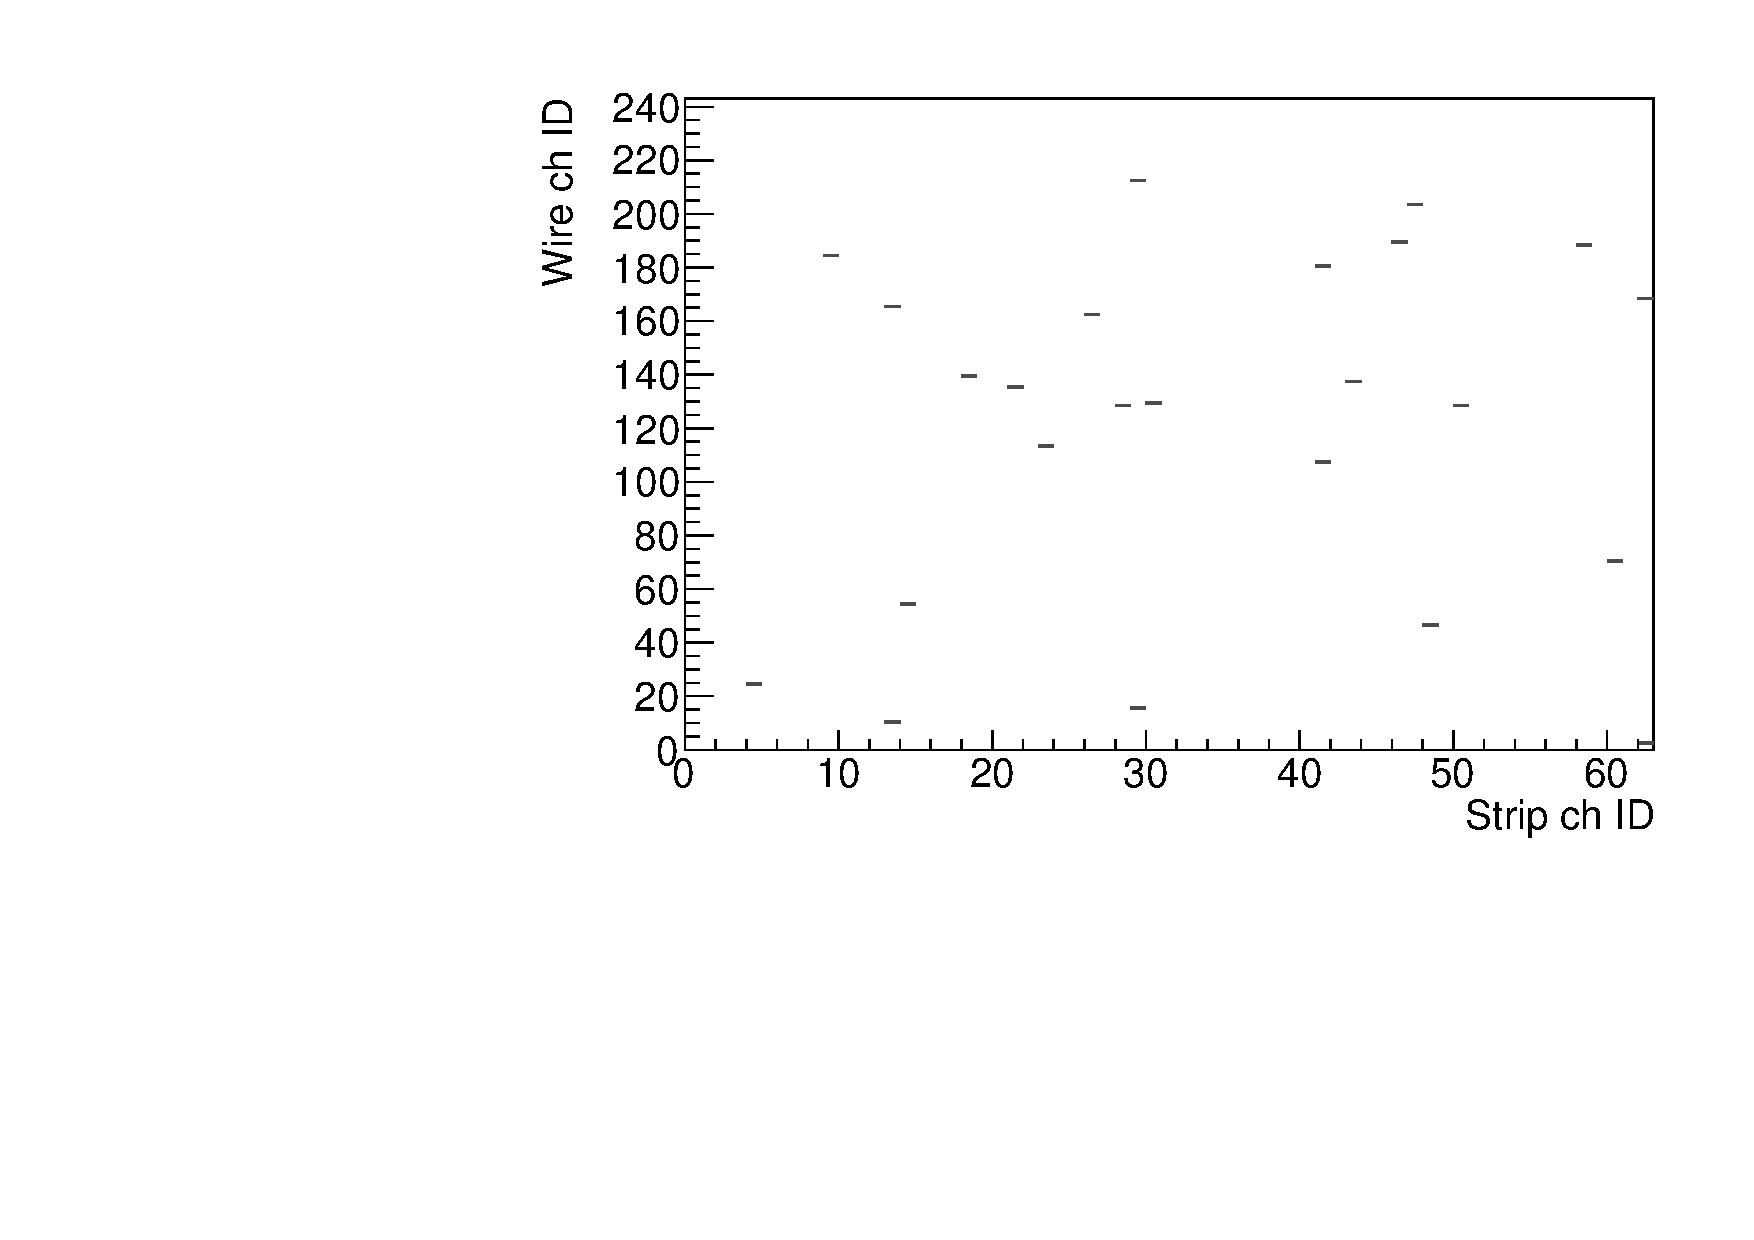
\includegraphics[height=6cm]{fig/Test/B_InfFW_wire.pdf}
          \subcaption{フォワード領域の結果}
      \end{minipage}
      \caption[異なる画像形式の比較]{無限運動量飛跡に対する、Wire Segment Reconstructionの応答。}
      \label{Inf_B_Wire}
  \end{figure}
  
  \begin{figure}
      \begin{minipage}[b]{.5\linewidth}
          \centering
          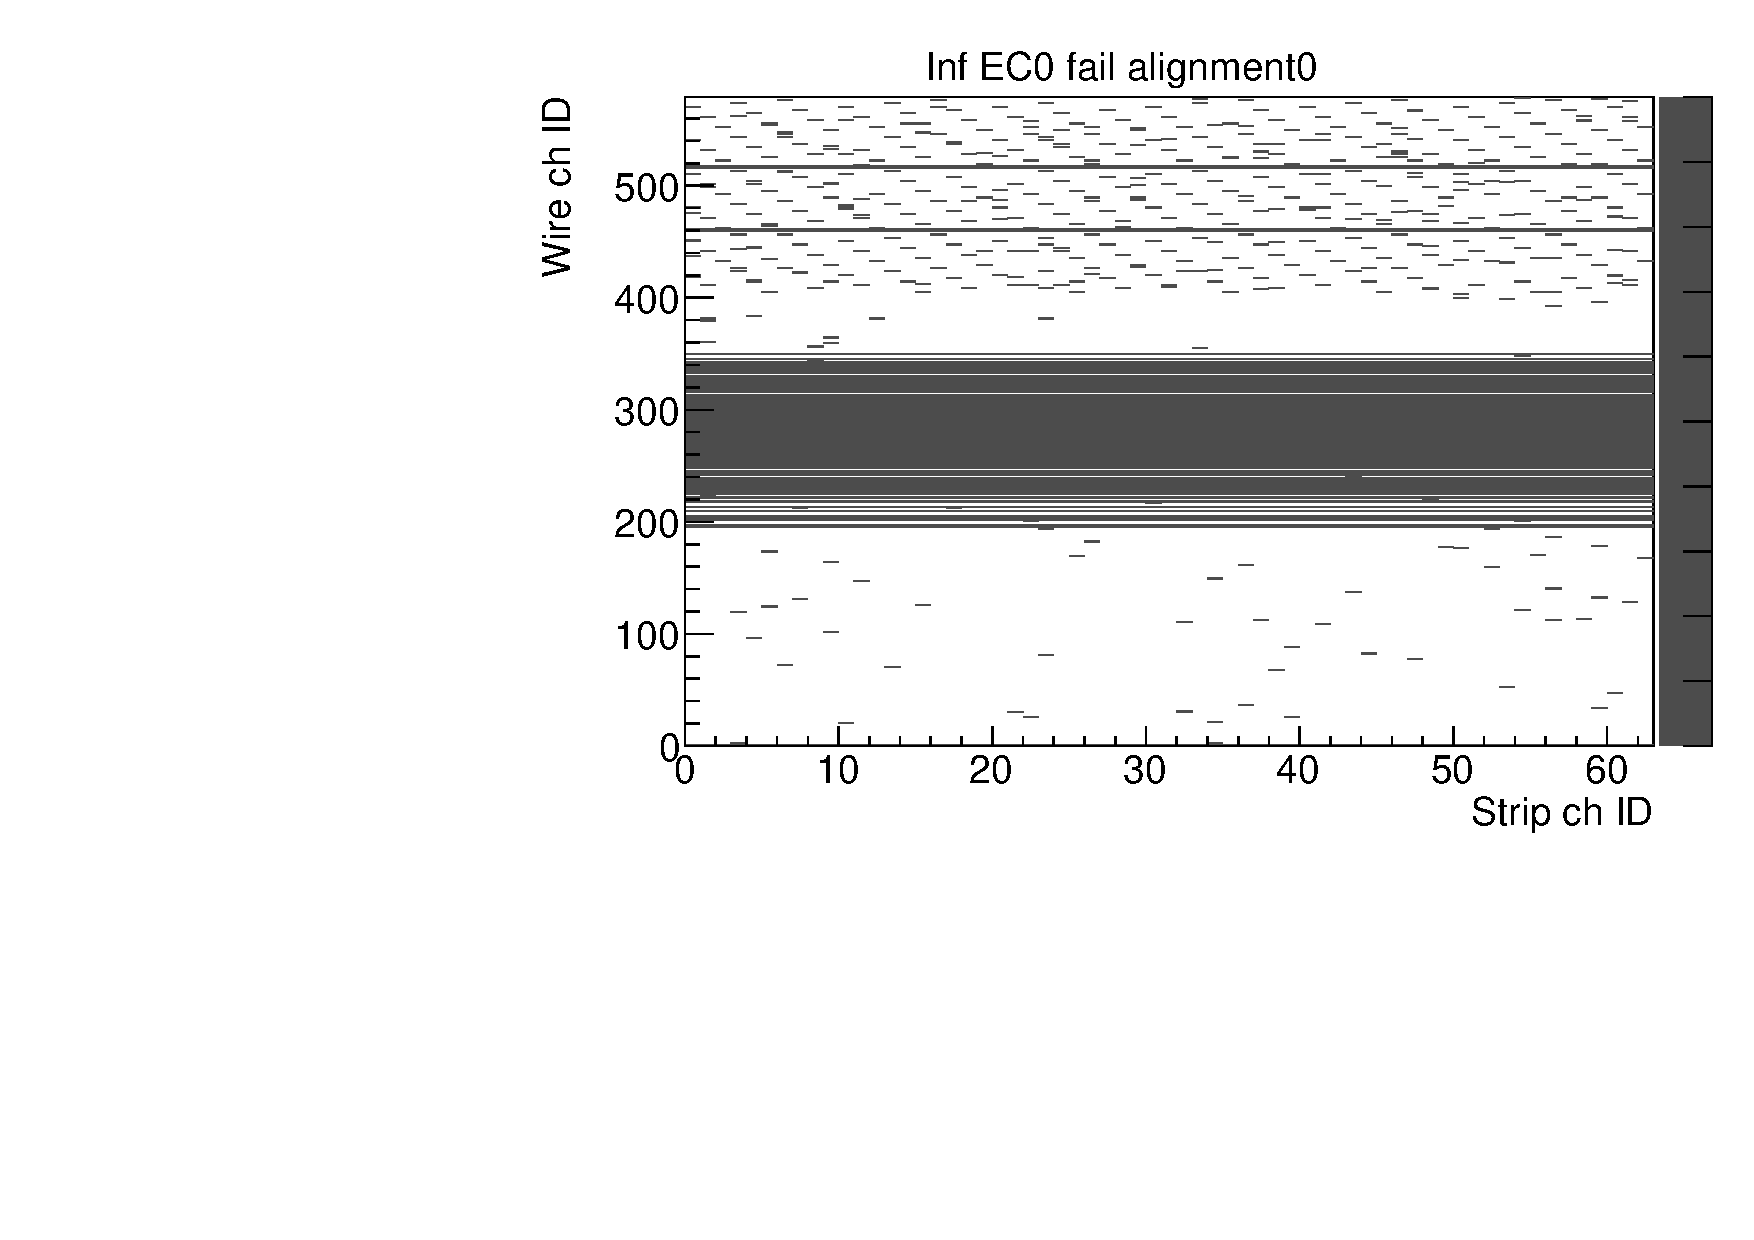
\includegraphics[height=6cm]{fig/Test/B_InfEC0_WS.pdf}
          \subcaption{エンドキャップ$\phi\,$0領域の結果}
      \end{minipage}
      \begin{minipage}[b]{.5\linewidth}
          \centering
          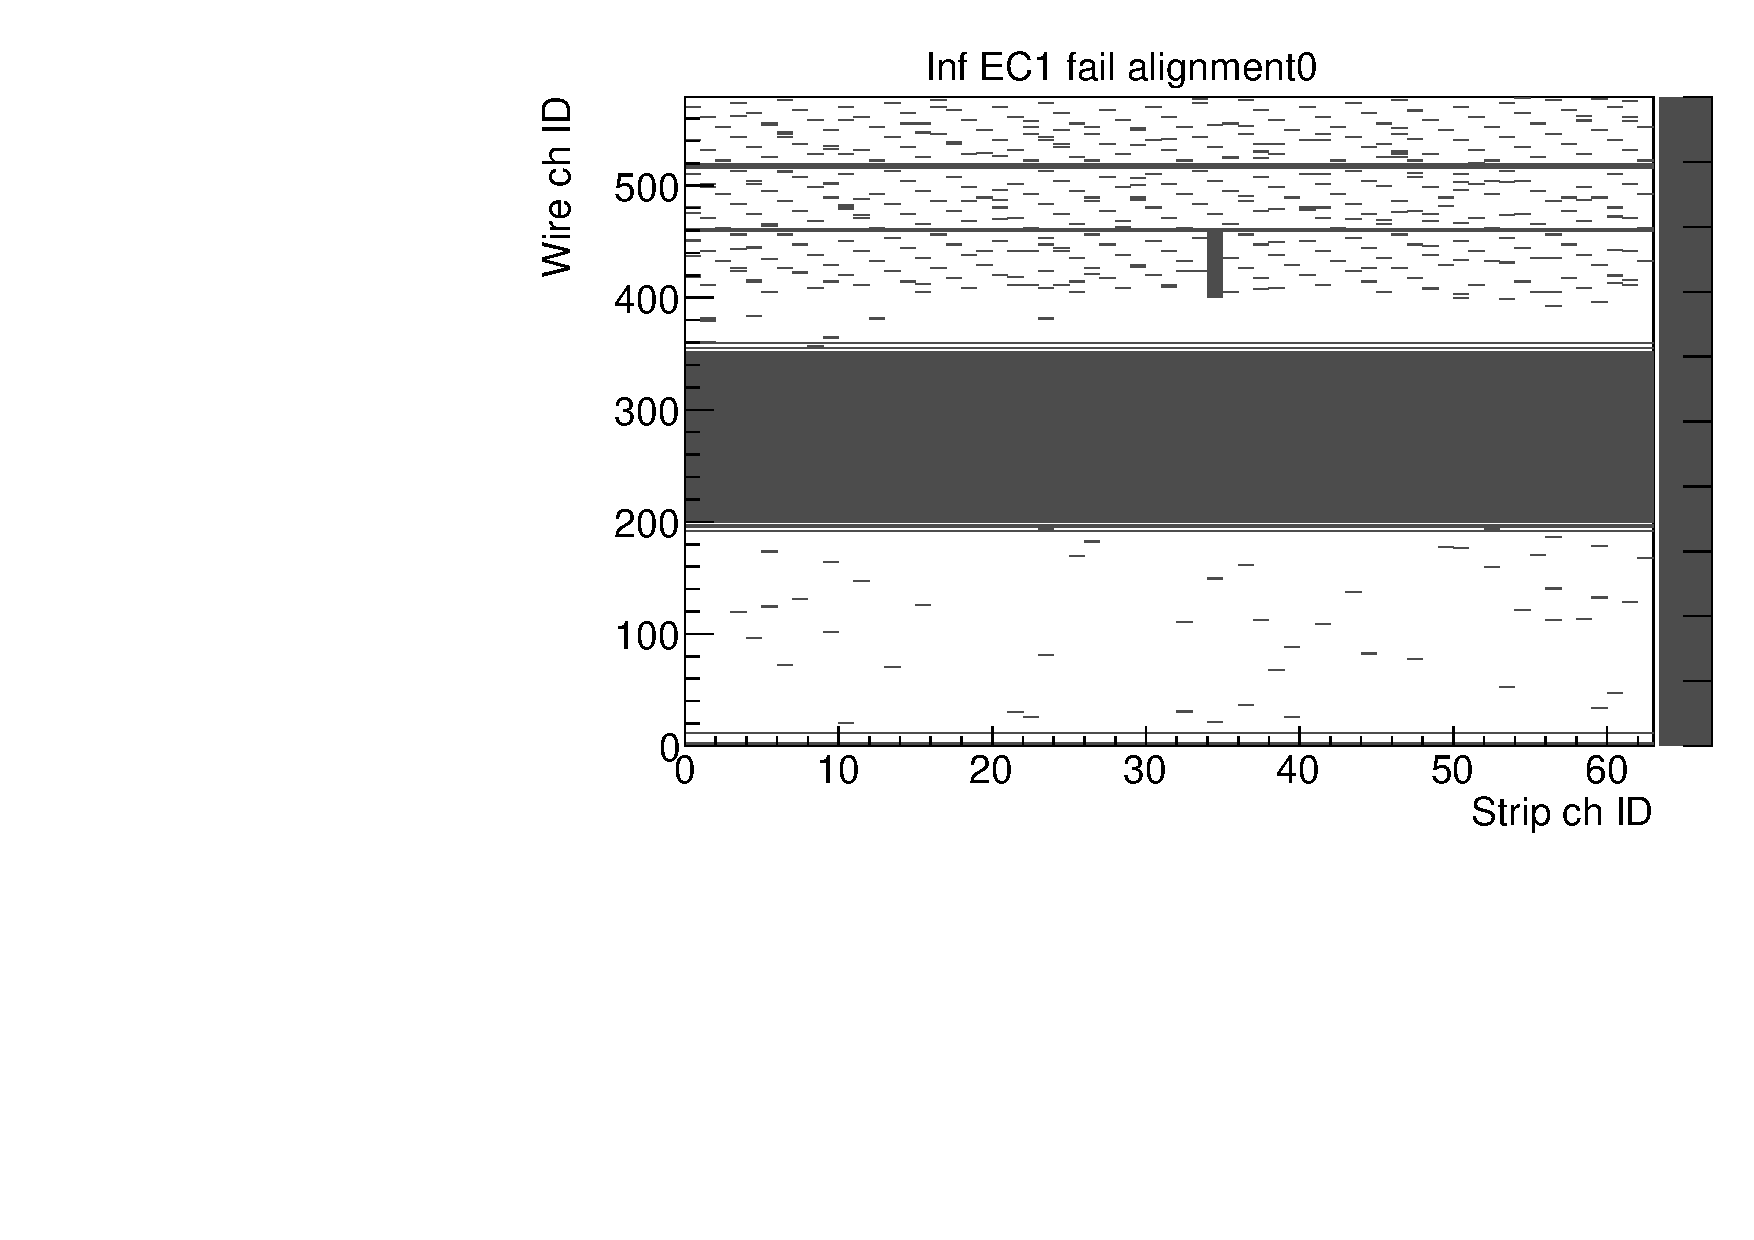
\includegraphics[height=6cm]{fig/Test/B_InfEC1_WS.pdf}
          \subcaption{エンドキャップ$\phi\,$1領域の結果}
      \end{minipage}\\
      \begin{minipage}[b]{\linewidth}
          \centering
          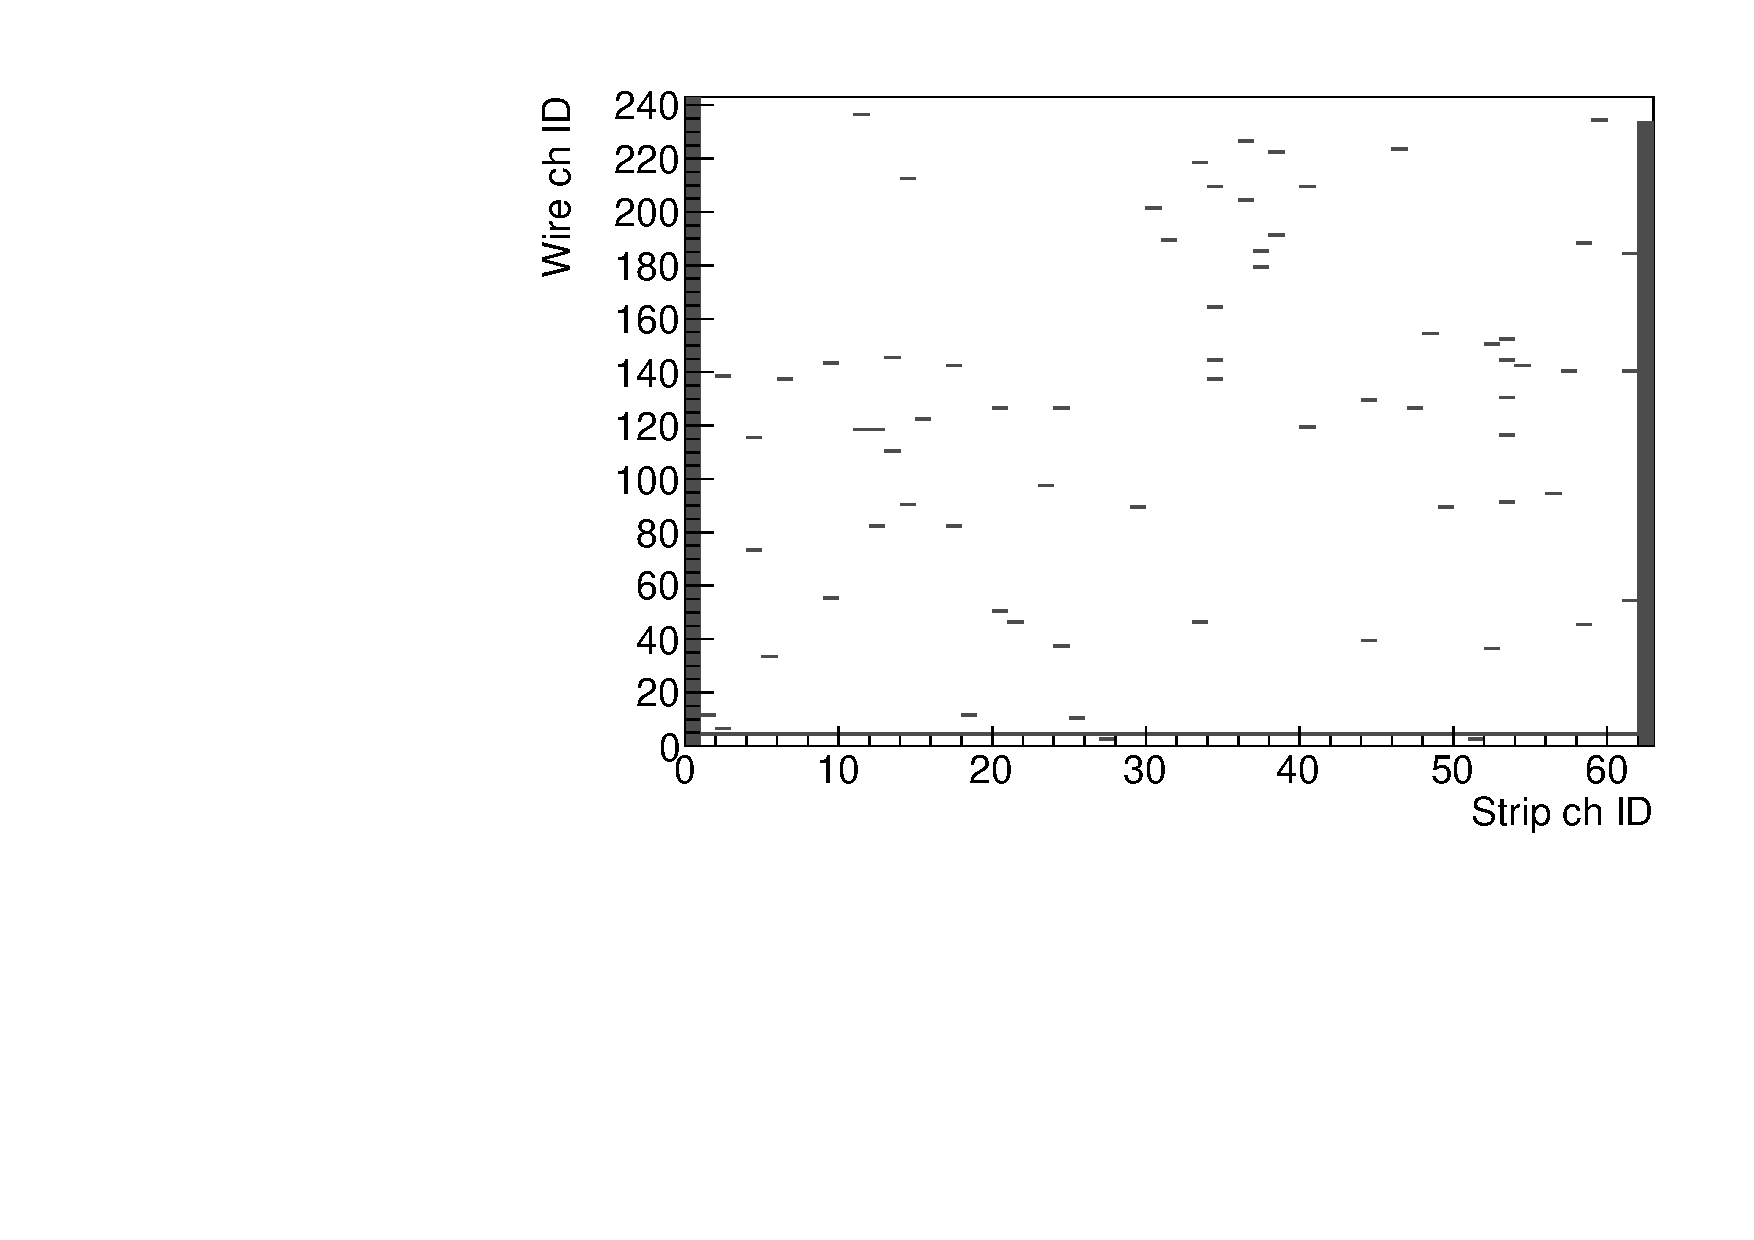
\includegraphics[height=6cm]{fig/Test/B_InfFW_WS.pdf}
          \subcaption{フォワード領域の結果}
      \end{minipage}
      \caption[異なる画像形式の比較]{無限運動量飛跡に対する、Wire Strip Coincidenceの応答。}
      \label{Inf_B_WS}
  \end{figure}

\paragraph{Strip Segment Reconstruction}  
\par
一方、FW領域ではStrip チャンネル番号0番、62番の全ての点で飛跡再構成に失敗している。この結果はBitwiseシミュレーターの結果と一致するものである。Bitiwiseシミュレーターを用いて詳細な調査を行ったところ、このInefficiencyはLUTに該当するチャンネルの飛跡候補が格納されていないことが原因であると理解され、修正が行われた。図\ref{Bitwise_example}にBitwiseシミュレーターの出力の例を示す。このログではStrip Station Coincidenceにおいて、M1、M2、M3で正しいスタッガード IDを出力できていること、Address Specifierで正しいAddressを生成できていること、LUTにアクセスした結果、あるはずの飛跡情報が格納されていなかった、ということが確認できる。これにより、Channel Mapping と Strip Station Coincidence は期待通り動作しているが、LUTから飛跡情報を取ってくる段階で失敗していることがわかった。

\begin{figure} 
  \centering
  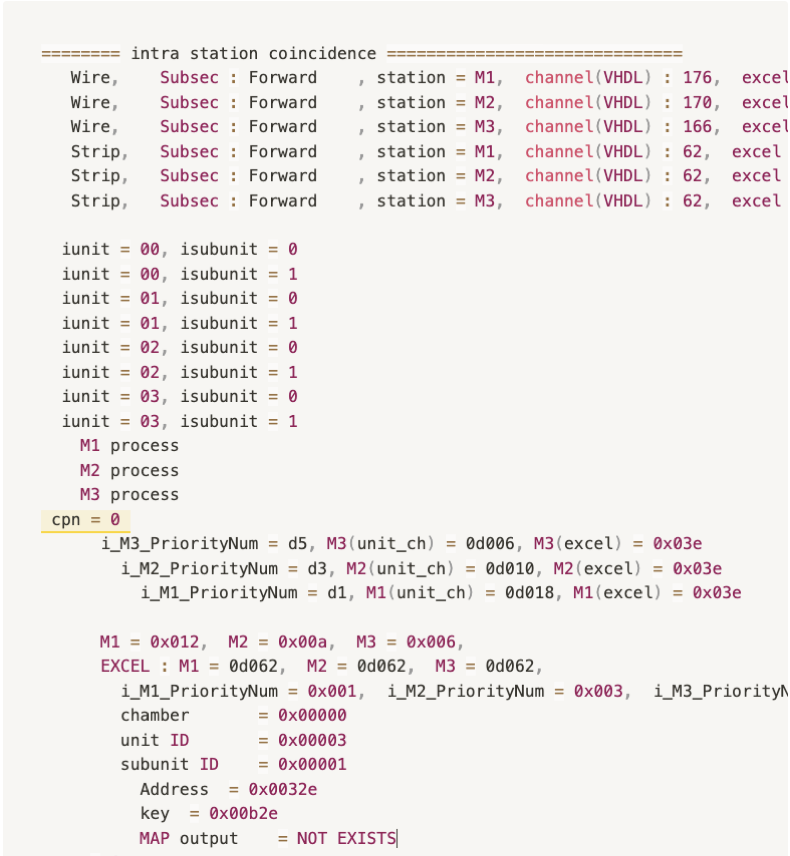
\includegraphics[width=16cm]{fig/Test/Bitwise_example.png}
  \caption[Strip Segment ReconstructionにおけるBitwiseシミュレーターのログ]{CStrip Segment ReconstructionにおけるBitwiseシミュレーターのログ}
  \label{Bitwise_example}
\end{figure}

このLUTのミスはソフトウェアシミュレーターで使われているrootファイル形式のものから、本番で使用するテキストファイル形式に整形する過程で生じたものである。そのため、ソフトウェアシミュレーターで検出することができず、本番とLUTを用いる実機試験で初めてわかった問題である。

\paragraph{Wire Segment Reconstruction}  
\par
Wire Segment Reconstructionではエンドキャップ領域の検出器の中心あたりで大きなInefficiencyが確認された。この不具合はスタッガードIDの割り振り方のミスによるものであると理解され、ケーブリングデータベースの修正が行われた。もともと、TGC検出器はステーションごとの$\eta$位置分解能が等しくなるように設計されており、設置によるずれが生じた後でも通し番号的にスタッガードIDを割り振れば同じ$\eta$をカバーするチャンネルを一意に定められると考えられていた。しかし、本実験の結果により、通し番号的にスタッガードIDを割り振ると、検出器の中央あたりの領域で$\eta$位置にずれが生じることが明らかになった。図\ref{Stag300}に通し番号的にスタッガードIDを振った時の各ステーションの$\eta$位置を示す。左にコインシデンスを取ることができたスタッガードID 100 ~ 105までの点を、右にコインシデンスを取ることができなかったスタッガーID 300 ~ 305の$\eta$位置を示す。通し番号的にスタッガードIDを振ると$\eta$が1.5 あたりの領域でステーションごとの$\eta$位置にずれが生じることがわかる。

\begin{figure}
\begin{minipage}[b]{.5\linewidth}
\centering
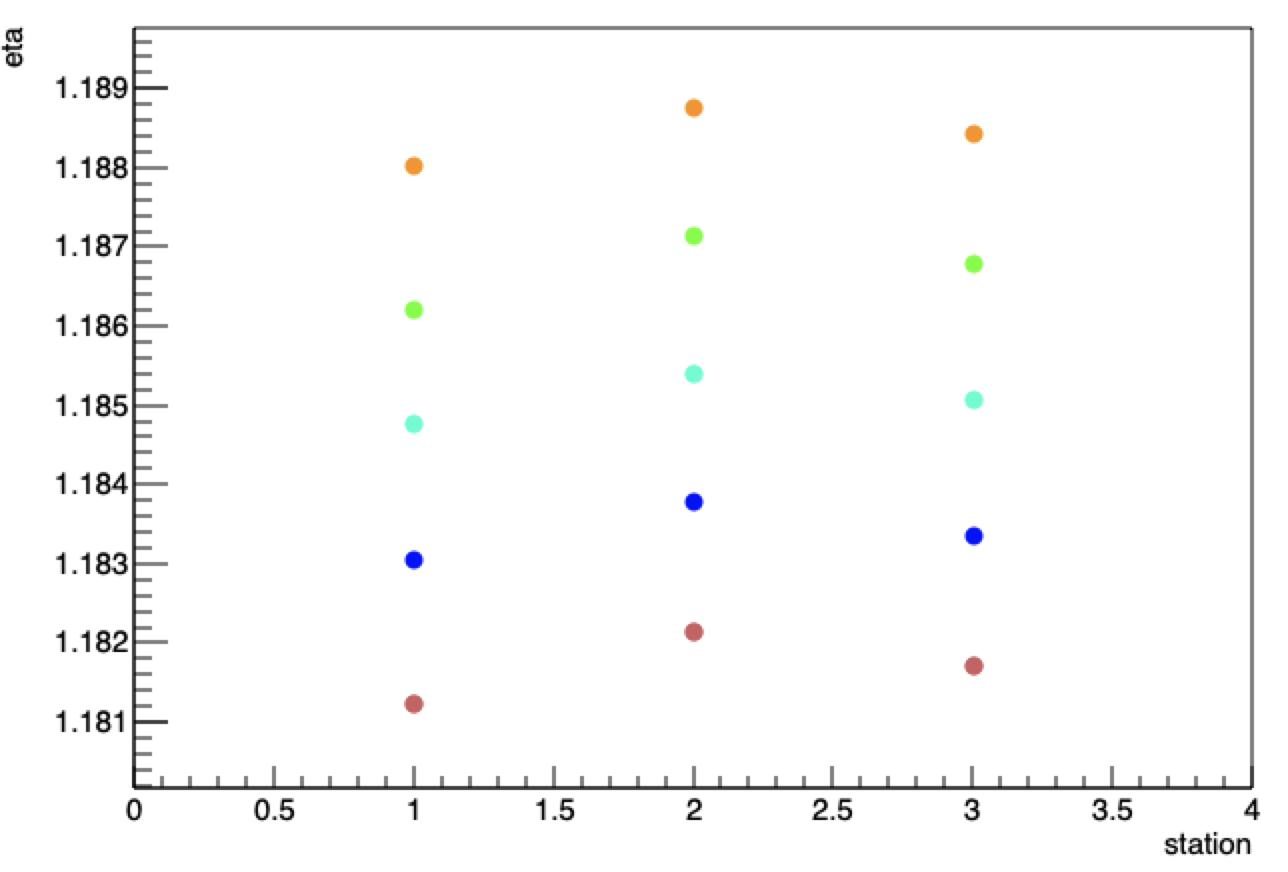
\includegraphics[height=5cm]{fig/Test/Stag100-105.png}
\subcaption{(a)}
\end{minipage}%
\begin{minipage}[b]{.5\linewidth}
\centering
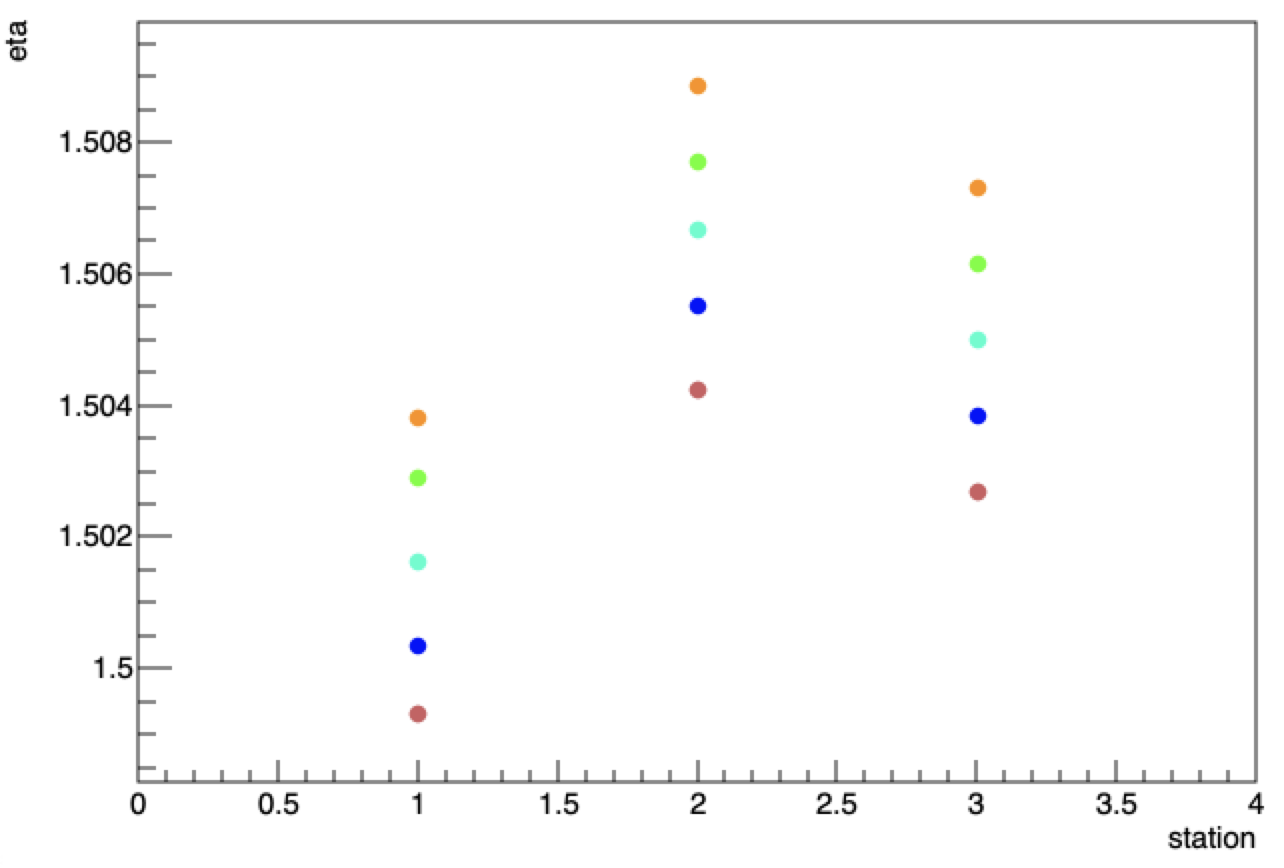
\includegraphics[height=5cm]{fig/Test/Stag300-305.png}
\subcaption{(a)}
\end{minipage}%
\caption[Wireでのスタッガードチャンネルのずれ]{Wireでのスタッガードチャンネルのずれ}
\label{Stag300}
\end{figure}

\paragraph{Wire Strip Coincidence}  
\par
Wire Strip CoincidenceではStrip、WireそれぞれのInefficiencyに加えて、未だ解決されていないWire スタッガードID 400 番以降の不具合が見えている。

\section{MCデータを用いた試験に際して行われたトリガーロジックの修正}
\label{sec:appendix:MC-test}
\paragraph{Wire Strip Coincidence}  
\par
シングルミューオンMCを用いた試験を始めた当初、Wire Strip Coincidenceで判定される\pt がtruth \pt と対応していないという問題があった。図\ref{pt_before}にWire LUT修正前の結果を示す。この図では横軸にtruth muonの\pt、縦軸にはWire Strip Coincidenceで判定された\pt を示す。本来であればであればtruth muonが5 - 10 GeVのイベントは\pt 閾値 5 GeV、10 - 15 GeV以上のものは10 GeV、とtruth ptに対応した\pt 閾値が出されるはずであるがそうなっていない。

\begin{figure} 
\centering
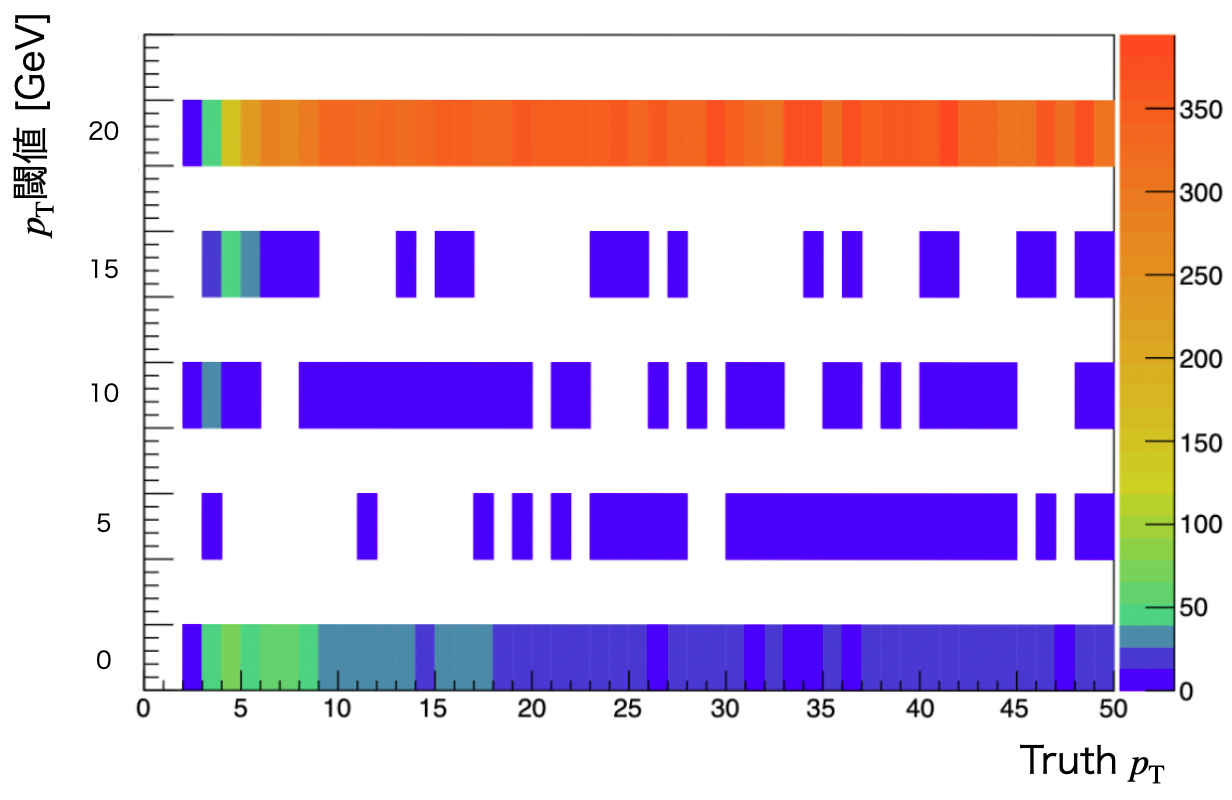
\includegraphics[width=16cm]{fig/Test/pt_before.png}
\caption[]{Wire LUT修正前のTruth $p_mathrm{T}$とWire Strip Coincidenceで判定された$p_mathrm{T}$の関係。}
\label{pt_before}
\end{figure}

問題のデバッグを行ったところ、Wire Segment Reconstructionの出力として定義される$\Delta\theta$の単位とWire Strip Coincidenceの入力として定義される$\Delta\theta$の単位が互いに異なっていた。Wire Segment reconstructionでは$\Delta\theta$は4 mrad区切りの整数値として出力される。一方、Wire Strip Coincidenceでは1.25 mrad区切りの整数値として解釈する。そのため、例えばTruthの$\Delta\theta$が10 mradの場合、Wire Segmnet Reconstructionは" $10 \mathrm{mrad} //4 = 2$ "という整数値を出力し、Wire Strip Coincidenceではそれを$1.25 \times 2 = 2.5 \mathrm{mrad}$と解釈してコインシデンスを行っていた。これによりTruthの\pt が小さく、$\Delta\theta$が大きいイベントに対しても高い\pt 閾値判定を行っていた。
この不具合の修正のため、Wire Strip Coincidenceの高い分解能に合わせる形でWire LUTを作り直した。その結果を図\ref{}に示す。期待通りの\pt 判定が行われるようになったことが見てとれる。
 
\begin{figure} 
\centering
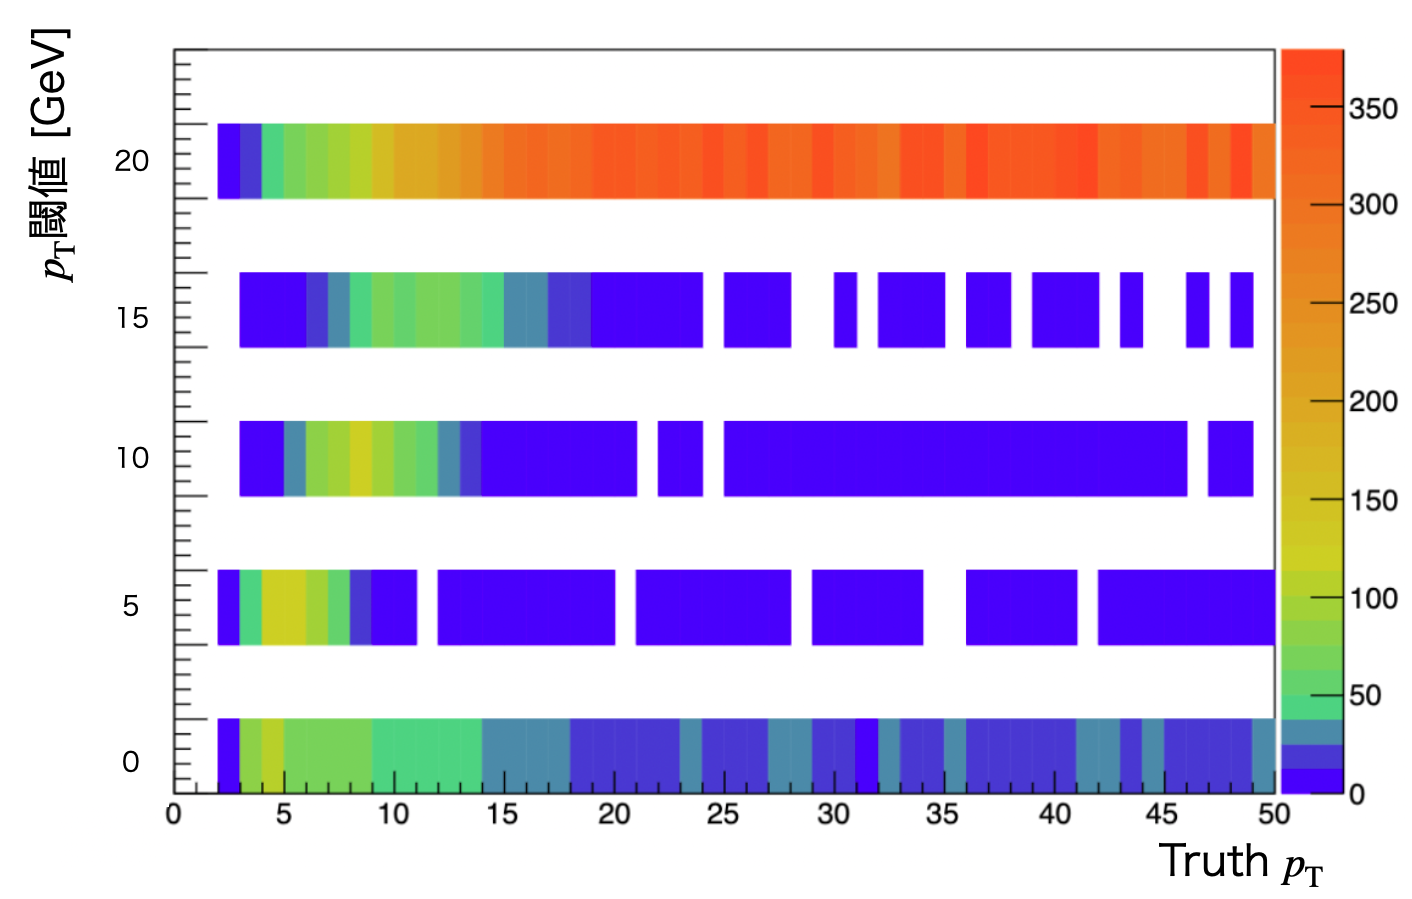
\includegraphics[width=16cm]{fig/Test/pt_after.png}
\caption[]{Wire LUT修正後のTruth $p_mathrm{T}$とWire Strip Coincidenceで判定された$p_mathrm{T}$の関係。}
\label{fig_CTA}
\end{figure}



\section{プラトー領域のInefficiencyの調査}
\label{sec:appendix:plateau}
図\ref{SM_A_WS_turnon}で示すようにシングルミューオンモンテカルロデータを利用すると、Truth Pt が 20 GeVより十分大きいプラトー領域においても6 \%程度のInefficiencyが見られる。本節ではこのInefficiencyの原因について考察する。
Inefficiencyの原因として主に以下の2つが考えられる。一つ目はTGC検出器のミューオン検出効率が100 \%ではないことによるInefficiencyである。高輝度LHC-ATLAS実験でのトリガーロジックはワイヤーでは7層中5層かつ各ステーションに少なくても1つヒットがあること、ストリップでは6層中4層かつ各ステーションに少なくても1つヒットがあること、が要求される。そのため例えばミューオンがM2の2層ともヒットを残さず、素通りしたとすると飛跡を再構成することはできない。2017年の運転におけるTGC各層のヒット検出効率分布を図\ref{tgchit_efficiency}に示す。1枚のガスレイヤーにおけるヒット検出効率の平均ははワイヤーで92.7 \%、ストリップで92.1 \%程度であることが知られている。

\begin{figure}
\begin{minipage}[b]{.5\linewidth}
\centering
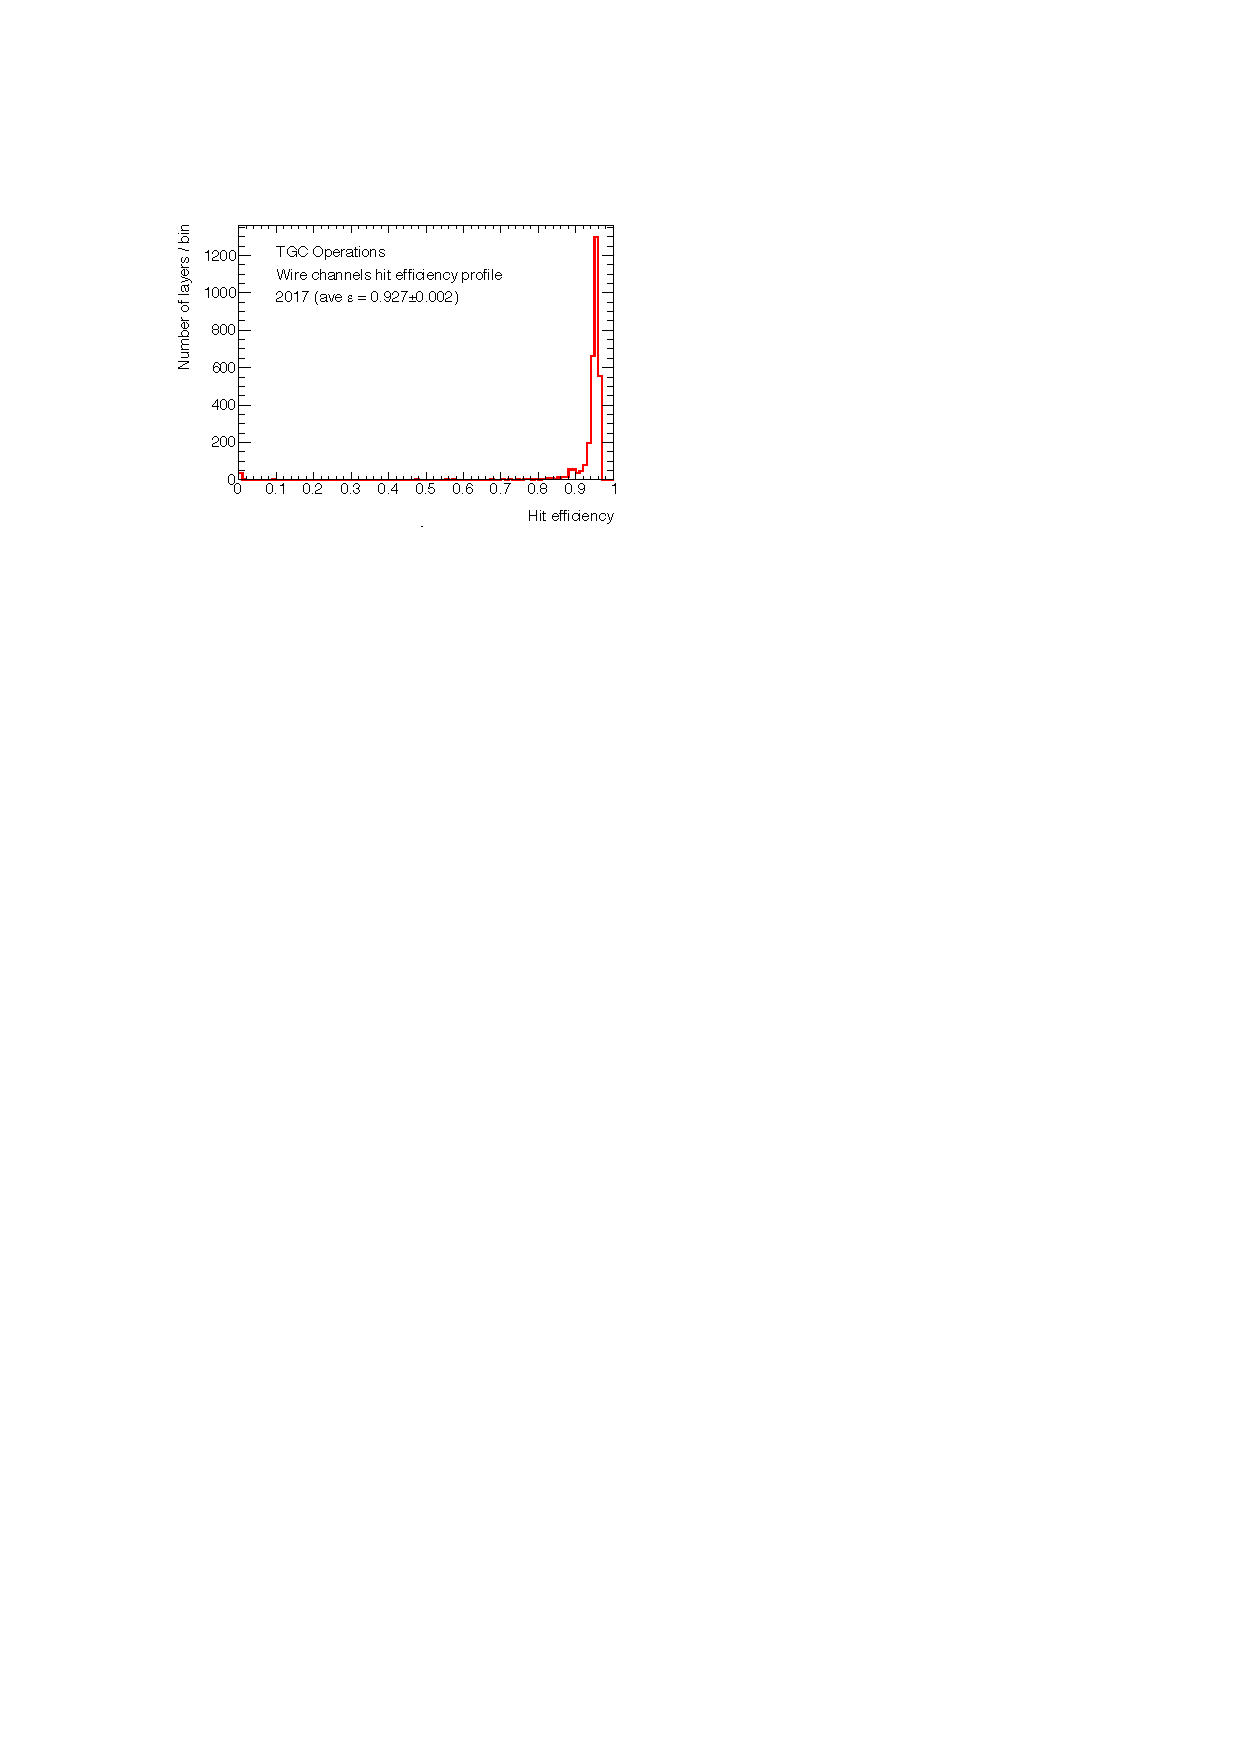
\includegraphics[height=5cm]{fig/Test/tgchit_wire.pdf}
\subcaption{ワイヤー}
\end{minipage}%
\begin{minipage}[b]{.5\linewidth}
\centering
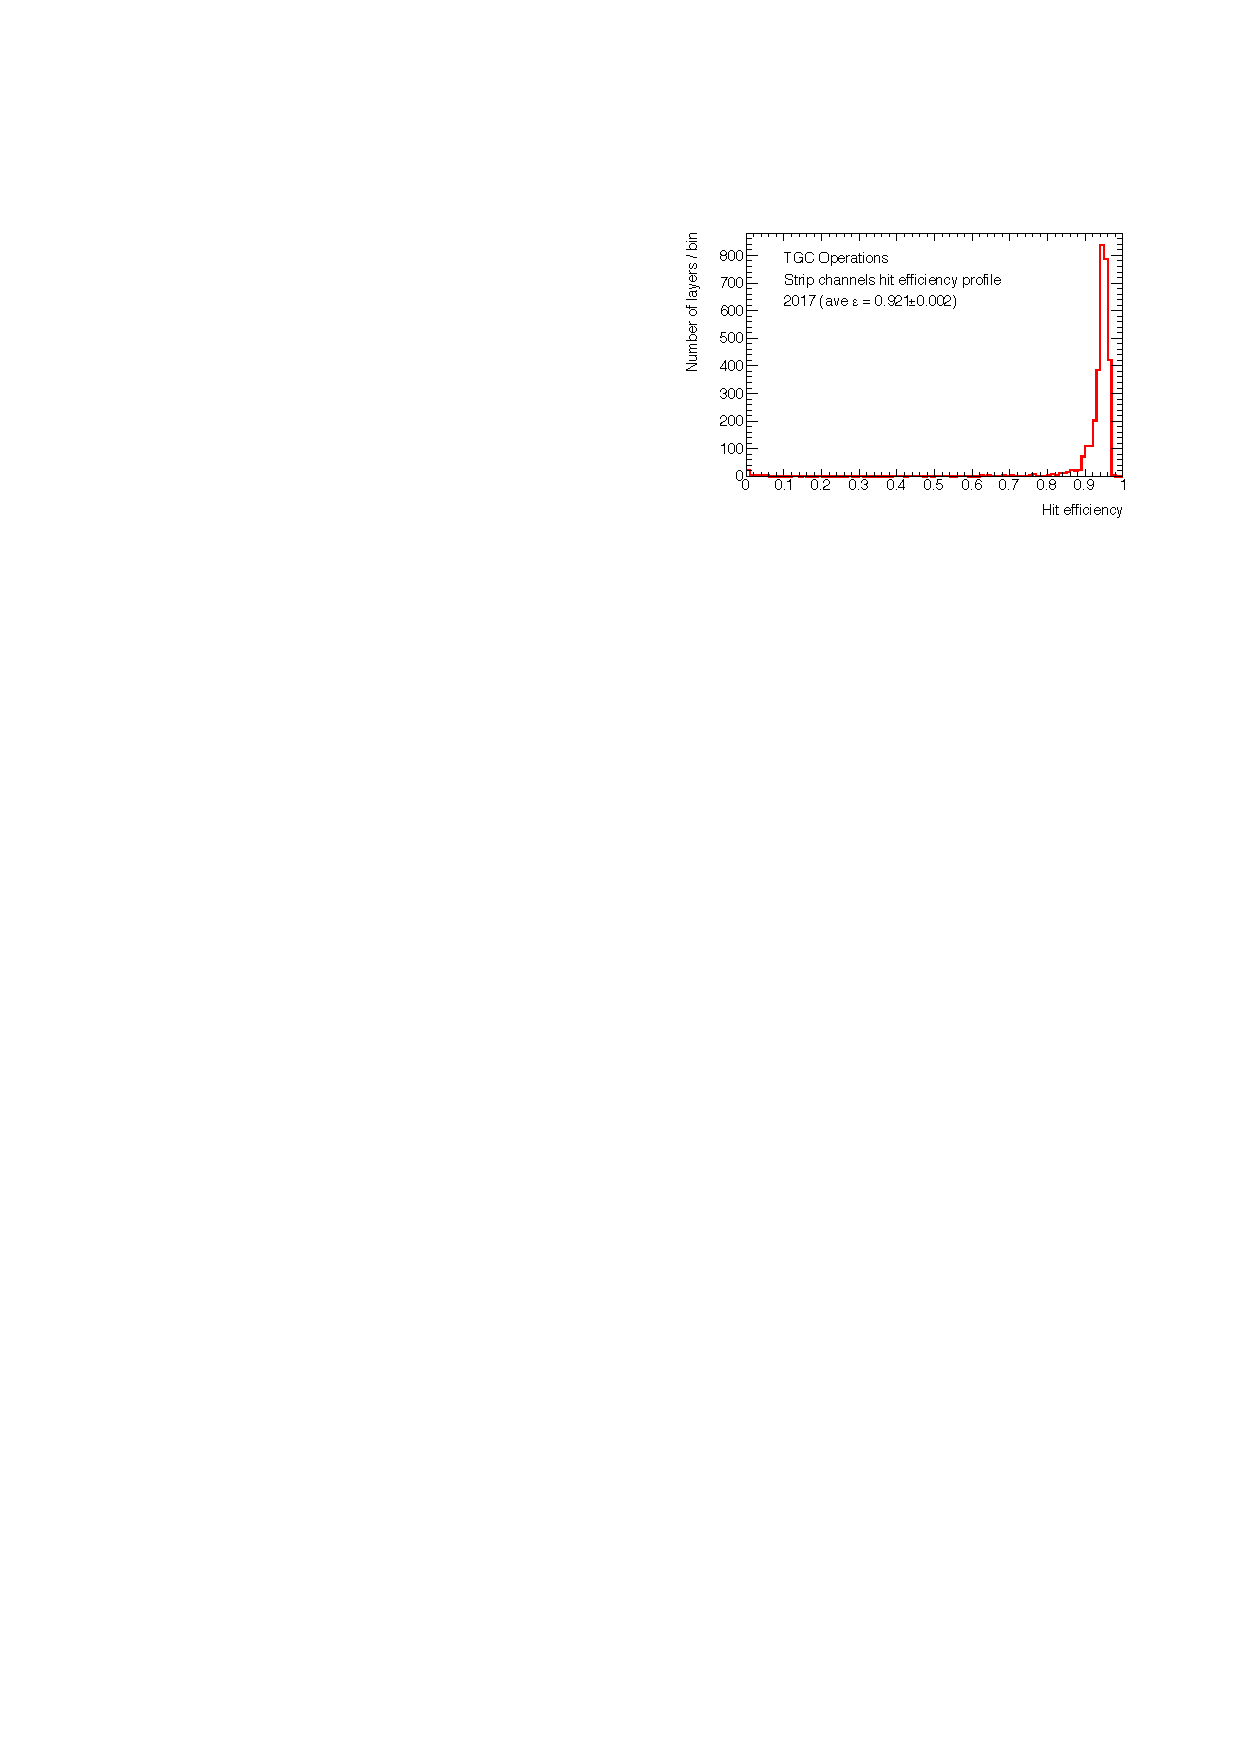
\includegraphics[height=5cm]{fig/Test/tgchit_strip.pdf}
\subcaption{ストリップ}
\end{minipage}%
\caption[2017年運転における TGC 各層のヒット検出効率]{2017年運転における TGC 各層のヒット検出効率\cite{mt_kawaguchi}}
\label{tgchit_efficiency}
\end{figure}

2つ目はTGC検出器にミューオンのヒット信号は検出されるが、多重散乱や制動放射に起因するInefficiencyである。多重散乱によりミューオン飛跡が途中で大角度に屈折したり、制動放射で生じた光子から電磁シャワーが生じ大量のヒットがTGCに残される場合には、Segment Reconstructionで正しい飛跡を再構成できなくなる。このようなイベントの例を図\ref{Brems}に示す。この図は実際のシングルミューオンモンテカルロサンプルに含まれる、TGCのヒット情報を3次元的にプロットしたものである。横軸と縦軸にヒットのあった座標位置、奥行き方向にTGCのレイヤー番号を示す。赤色の点がWireのヒットで青色がStripのヒット情報を表す。このイベントでは3層目でミューオンが制動放射を起こし、それに起因する電磁シャワーが4層目以降に複数のヒットを残していると推測される。

\begin{figure} 
\centering
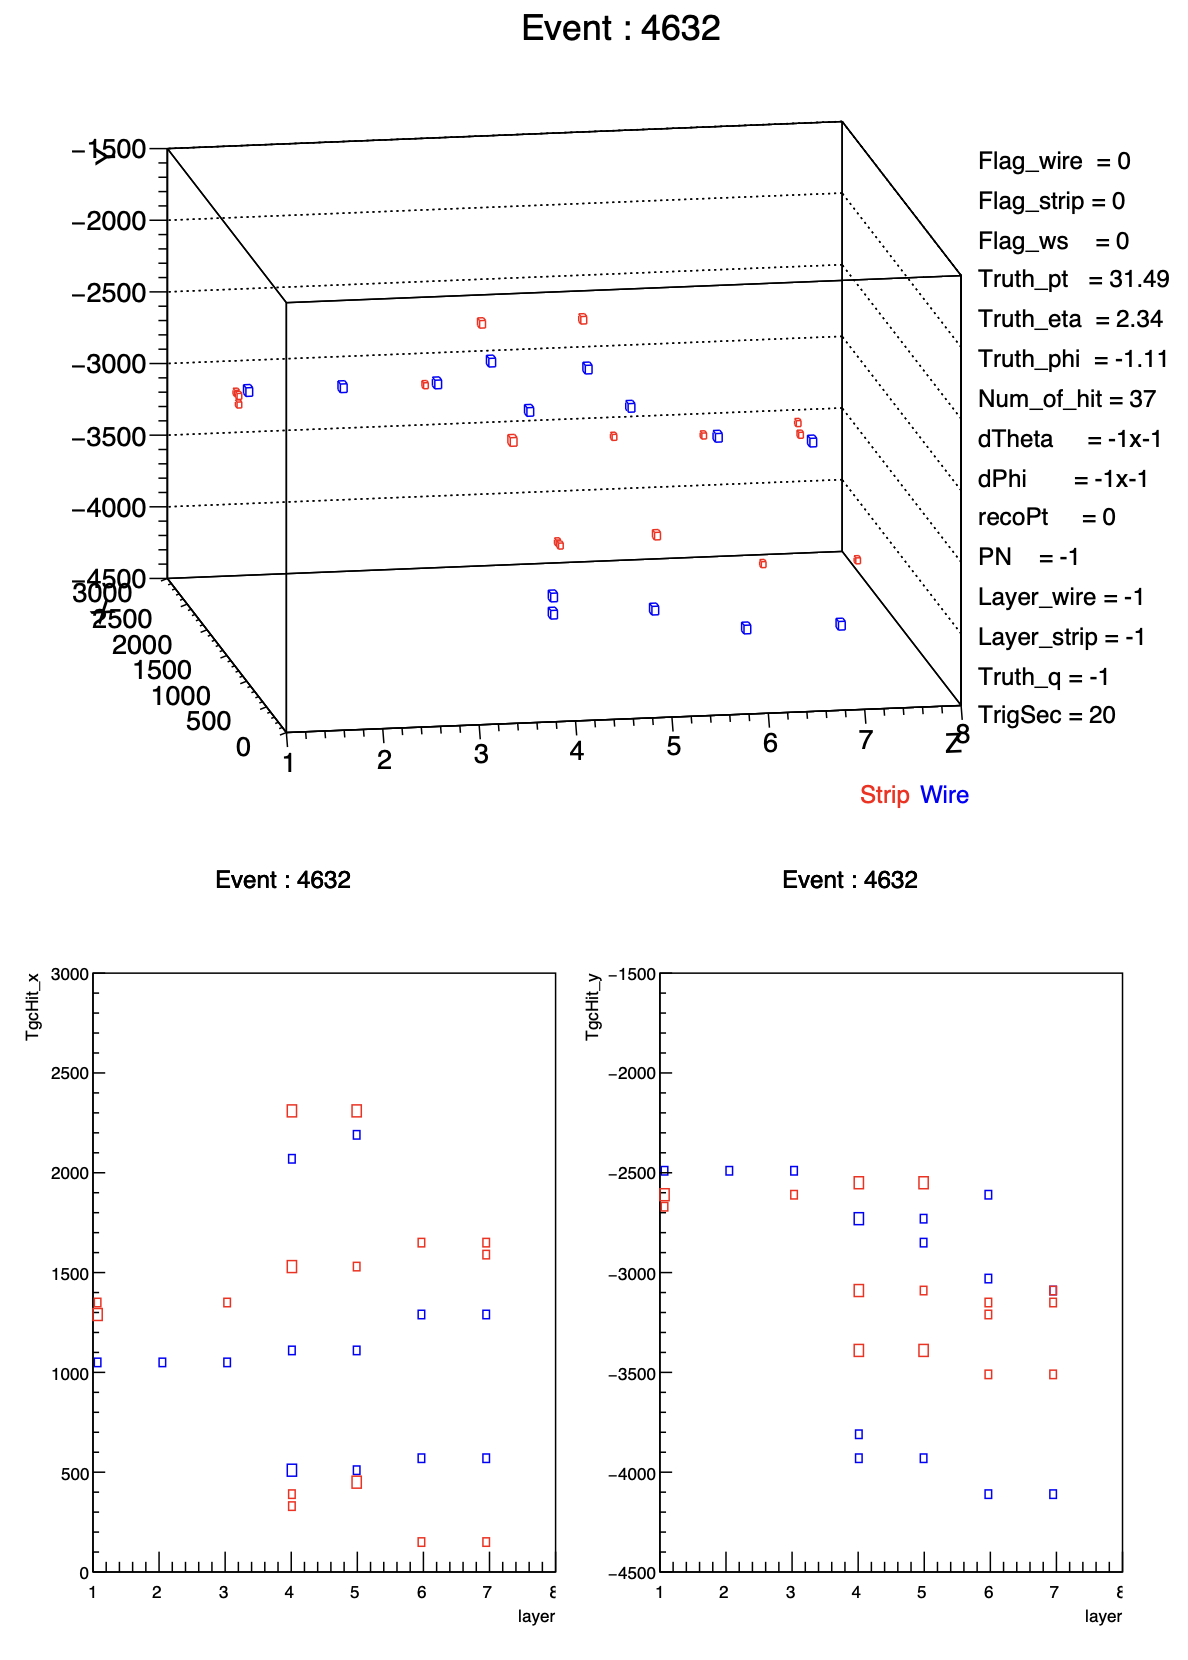
\includegraphics[width=16cm]{fig/Test/Brems.png}
\caption[制動放射が生じたと思われるイベントディスプレイ]{制動放射が生じたと思われるイベントディスプレイ}
\label{Brems}
\end{figure}

Wire Strip Coincidenceで見られた6 \%のInefficiencyがどのような理由で生じているか調査するため、実機試験で落ちたイベントに対してイベントディスプレイを作成し、アイスキャンを行った。

データセットとして、フォワード領域のシングルミューオンイベントを10,000イベント用意した。このうちWire Strip Coincidenceで飛跡再構成に失敗したイベントは合計 583 イベントだった。
アイスキャンによる落ちた原因の調査結果を表\ref{tab:eyscan}に示す。結果、プラトー領域における6 \%程度のInefficiencyのうち3割はヒットレイヤーが少ないことが原因、もう3割は多重散乱や制動放射により正しく飛跡を再構成することが困難なイベント、残りの4割は原理的な困難はなくLUTの調整などにより解決できる可能性があるものであるとわかった。

\begin{table}[]
  \centering
  \caption{Wire Strip Coincidenceで飛跡再構成に失敗したイベントの調査結果}
  \label{tab:eyscan}
  \begin{tabular}{|c|c|}
  \hline
  飛跡再構成の原因                        & イベント数       \\ \hline\hline
  ヒットを残したレイヤーが少なく原理的に飛跡再構成ができないもの & 169 / 10000 \\ \hline
  多重散乱や制動放射により正しく飛跡を再構成することが困難なもの & 181 / 10000 \\ \hline
  その他 (アイスキャンでは原因を判断できなかったものを含む)  & 233 / 10000 \\ \hline
  合計                              & 583 / 10000 \\ \hline
  \end{tabular}
\end{table}


% \section{アライメントのずれに対するInefficiencyの考察}
% \label{sec:appendix:alignment}
% モンテカルデータはTGC検出器が、設計通りの理想位置に設置されていることを仮定して作成されたデータセットである。しかし、実際のTGC検出器はアライメントのずれにより、理想位置からずれた位置に設置されている。年度末のメンテナンス期間にはTGC検出器は一時移動し、再設置されるため、その度ごとにアライメントのずれが生じる。TGCトリガーロジックではチャンネルのヒット位置をもとに角度情報を算出するため、このアライメントのずれは角度再構成や\pt 再構成に影響を与える。特にその影響が顕著なWire Segment Reconstructionではこのずれを吸収するために、アライメントが行われるごとに新しくLUTを作成する予定である。しかし、これまでにアライメントのずれがどれだけトリガー性能に影響を与えるか評価されたことがない。
% そこで本研究では、シングルモンテカルロデータを用いて、アライメントのずれを考慮した場合と、考慮しない場合でどれだけ検出効率に差が生じるか測定した。
% 具体的には理想位置のジオメトリをもとに作成されたシングルミューオンイベントに対し、理想位置のジオミトリをもとに作成したLUTを使用してWire Segment Reconstructionを走らせた場合とと、2022年のアライメント後のジオミトリ情報をもとに作成したLUTを使用した場合とを比較する。

% 図\ref{alignment_wire}にWire Segment Reconstruction検出効率を示す。
% アライメントのずれを考慮した場合と考慮しない場合で、数\%程度検出効率に差が生じることがわかった。特に、フォワード領域ではジオミトリのずれによるInefficiencyが顕著な様子が窺える。

% \begin{figure} 
% \centering
% 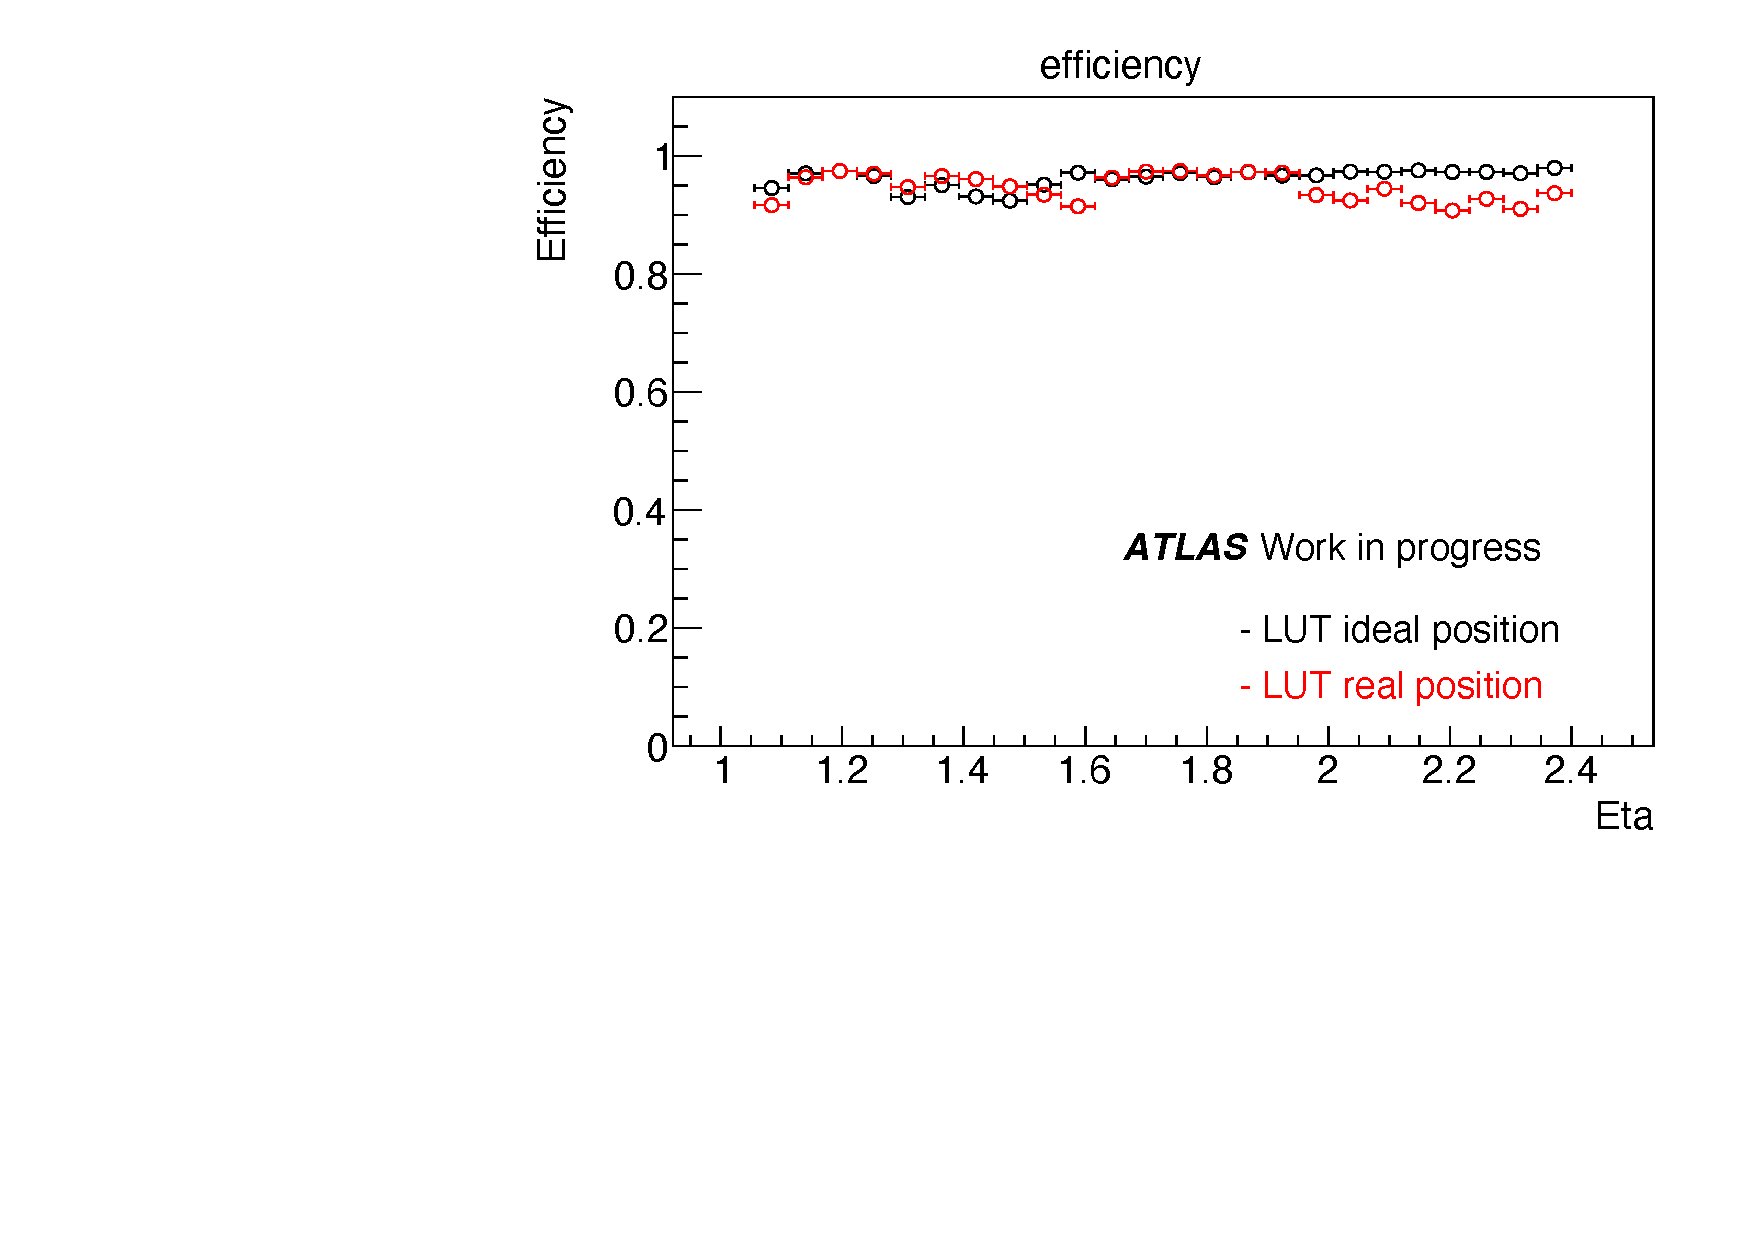
\includegraphics[width=16cm]{fig/Test/alignment_wire.pdf}
% \caption[]{理想位置のジオミトリを仮定したLUTと、2022年の実際のアライメントを考慮した場合のWire Segment Reconstructionの飛跡再構成効率の比較}
% \label{alignment_wire}
% \end{figure}

% 図\ref{alignment_ws}にWire Strip Coincidenceの\pt 閾値20 GeVに対するトリガー効率を示す。アライメントを考慮したLUTではTruth Muon \pt が20 GeVより小さいイベントに対して、不当に高い検出効率を持ってしまっていることがわかる。これはアライメントのずれによる角度再構成の不正確さが、角度を本来よりも小さく見積もる方向に働いた結果であると推測される。このように\pt 分解能が落ちると、物理的に興味のある\pt が高いイベントのみを選択するというトリガー本来の役割を果たせない。
% この結果では、アライメントを考慮したLUTを作成することが必要であると結論付けられる。

% \begin{figure} 
% \centering
% 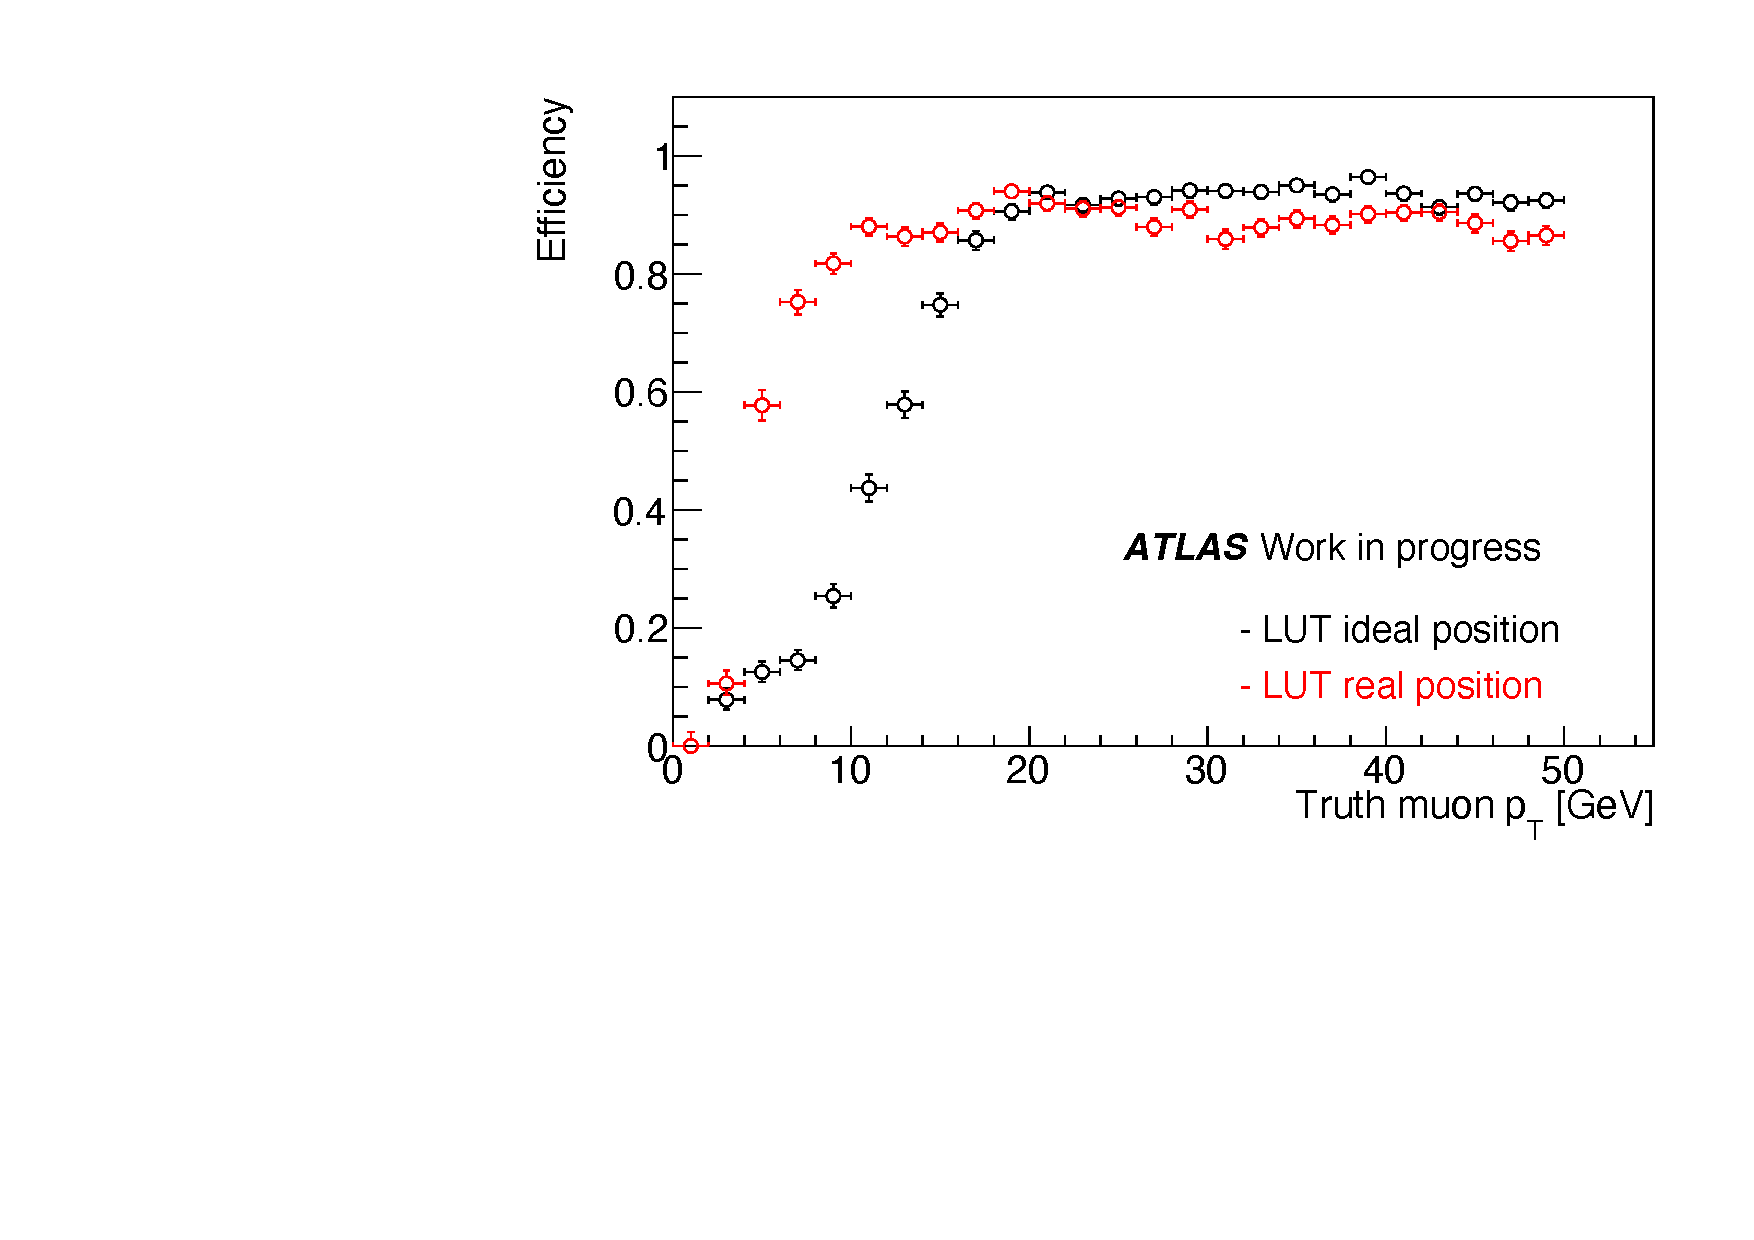
\includegraphics[width=16cm]{fig/Test/alignment_ws.pdf}
% \caption[CTAの完成想像図]{理想位置のジオミトリを仮定したLUTと、2022年の実際のアライメントを考慮した場合のWire Strip Coincidenceの飛跡再構成効率の比較}
% \label{alignment_ws}
% \end{figure}


